\documentclass[11pt,a4paper]{article}

\usepackage[utf8]{inputenc}
\usepackage[T1]{fontenc}
\usepackage{lmodern}
\usepackage[english]{babel}
\usepackage{geometry}
\usepackage{graphicx}
\usepackage{float}
\usepackage{caption}
\usepackage{amsmath}
\usepackage{amssymb}
\usepackage{booktabs}
\usepackage{xcolor}

\geometry{margin=1in}
\raggedbottom
\emergencystretch=3em

\title{\textcolor{red}{SCRATCH -- PRELIMINARY, ONE SEED EACH -- NOT PART OF THE FINAL REPORT} \\
       Report IX: does the completion signal need the rich path\_union mix, and do endpoints
       matter?}
\author{}
\date{Generated \today}

\begin{document}
\maketitle

\begin{center}
\fbox{\parbox{0.9\textwidth}{\centering\bfseries
This is a throwaway working document, not the Report~IX manuscript. Every experiment here is a
single seed (seed $1000$) -- exactly why these results live here and not in the real report: we
always want several seeds before trusting a number as a real result, and these are not yet
replicated. Nothing here should be copied into the real Report~IX manuscript until more seeds
are in.}}
\end{center}

\section*{What this is}

Three new training runs, one seed each, $n=46$, similarity read-out, RoBERTa-faithful $L=2$
single-head $d_{\mathrm{model}}=512$, $10^6$ online steps, batch $1000$ -- identical setup to
every other training in this report, only the training \emph{distribution} changes:

\begin{itemize}\setlength\itemsep{0.15em}
  \item \textbf{2-chains-only}: every training sample is a random two-way split of the $46$
        nodes into two disjoint paths (the short-component size drawn uniformly $1..45$ every
        sample) -- never the richer $1$--$4$-path path\_union mixture used everywhere else in
        this project since Report~VI.
  \item \textbf{1+2-path}: every sample is, with equal probability, either a single $46$-node
        chain (the $k{=}1$ case) or the same random two-way split as above -- a narrower mixture
        than path\_union (which also draws $3$- and $4$-component splits), spanning exactly the
        two cases path\_union itself draws most often.
  \item \textbf{2-cycles-only}: the same random two-way split as the first condition, but each
        segment closed into a cycle instead of left as an open path (so neither component has a
        degree-$1$ endpoint) -- the direct training-side analogue of Report~VIII's two-cycles
        test, which only ever evaluated a model that had \emph{never} seen a cycle in training.
\end{itemize}

All three are evaluated in-distribution with the same split-sweep battery used throughout this
project: the behavioural sweep (exact match, reach, cut, predicted-positive rate), the raw
pre-bias pre-scale similarity logit by pair type, the real attention scores/$\alpha$, and the
five-stage layerwise similarity geometry ($Z=\mathrm{scale}\cdot\cos+\mathrm{bias}$, connected
$>0$/disconnected $<0$ at every stage). For the two chain-based conditions the sweep runs
$a=1\,..\,23$; for the cycle condition it starts at $a=3$ (a cycle needs at least $3$ nodes).

\clearpage
\section{2-chains-only training}

\paragraph{Result: the endpoint-completion signal reproduces exactly, with a cleaner cut than
path\_union.} Exact match is $1.000$ for every split $a\le11$, then collapses to $0.000$ at
\emph{exactly} $a=12$ -- the same break point already seen for the full path\_union mixture at
this canvas size (\S sec:planpre). Reach in the long component drops to $0.79$ at the break and
then recovers smoothly to $0.96$ by the balanced split, closely mirroring path\_union's own
recovery shape. The one clear difference: \textbf{cut stays at $1.000$ across the entire sweep,
never dropping below $0.96$ even at the fully balanced split} -- path\_union-trained models
degrade to $\approx0.63$ cut at the same canvas (\S sec:planA). A single, narrow, explicitly-named
training distribution reproduces the same completion signal the richer $1$--$4$-path mixture
does, and if anything with a more robust cut.

\begin{table}[H]\centering\small
\begin{tabular}{ccccc}
\toprule
$a$ & exact & reach(long) & reach(short) & cut \\
\midrule
1--11 & 1.000 & 1.000 & 1.000 & 1.000 \\
\textbf{12} & \textbf{0.000} & \textbf{0.786} & 1.000 & 1.000 \\
15 & 0.000 & 0.832 & 1.000 & 1.000 \\
18 & 0.000 & 0.881 & 1.000 & 1.000 \\
20 & 0.000 & 0.914 & 0.995 & 1.000 \\
23 & 0.000 & 0.961 & 0.961 & 1.000 \\
\bottomrule
\end{tabular}
\caption{Split sweep $(a,46{-}a)$, seed $1000$ only, trained ONLY on random two-chain splits.
Selected rows ($a=1..11$ collapsed since all identical); full sweep in the figure below.}
\end{table}

\begin{figure}[H]\centering
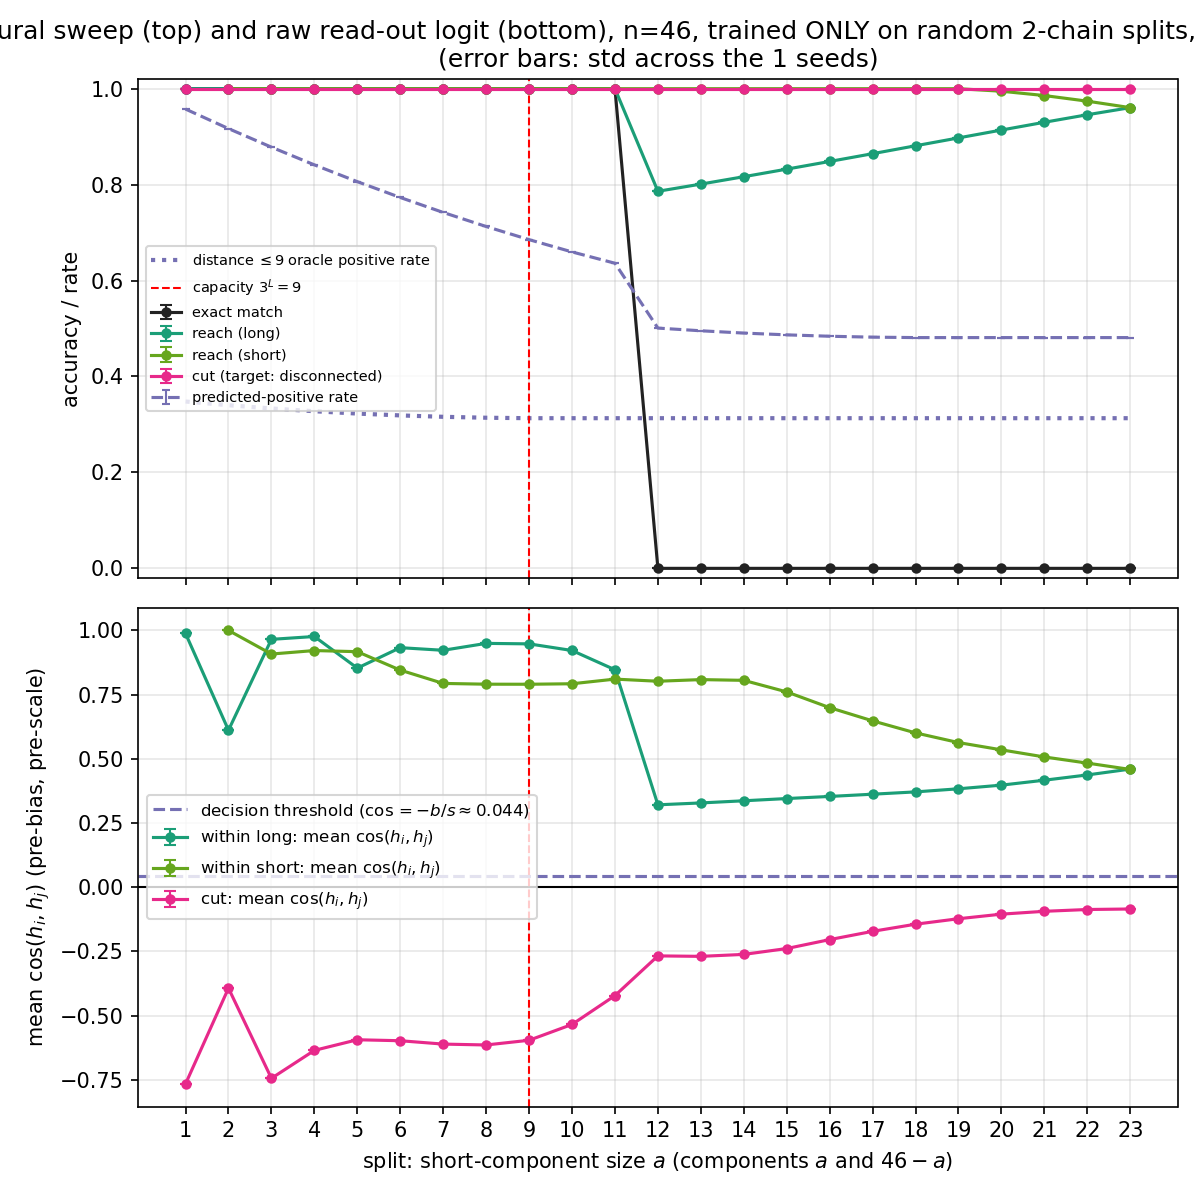
\includegraphics[width=0.95\textwidth]{figs/r9_sweep_and_logit_n46_splitchains.png}
\caption{Full sweep + raw similarity logit, seed $1000$, trained only on random two-chain
splits.}
\end{figure}

\begin{figure}[H]\centering
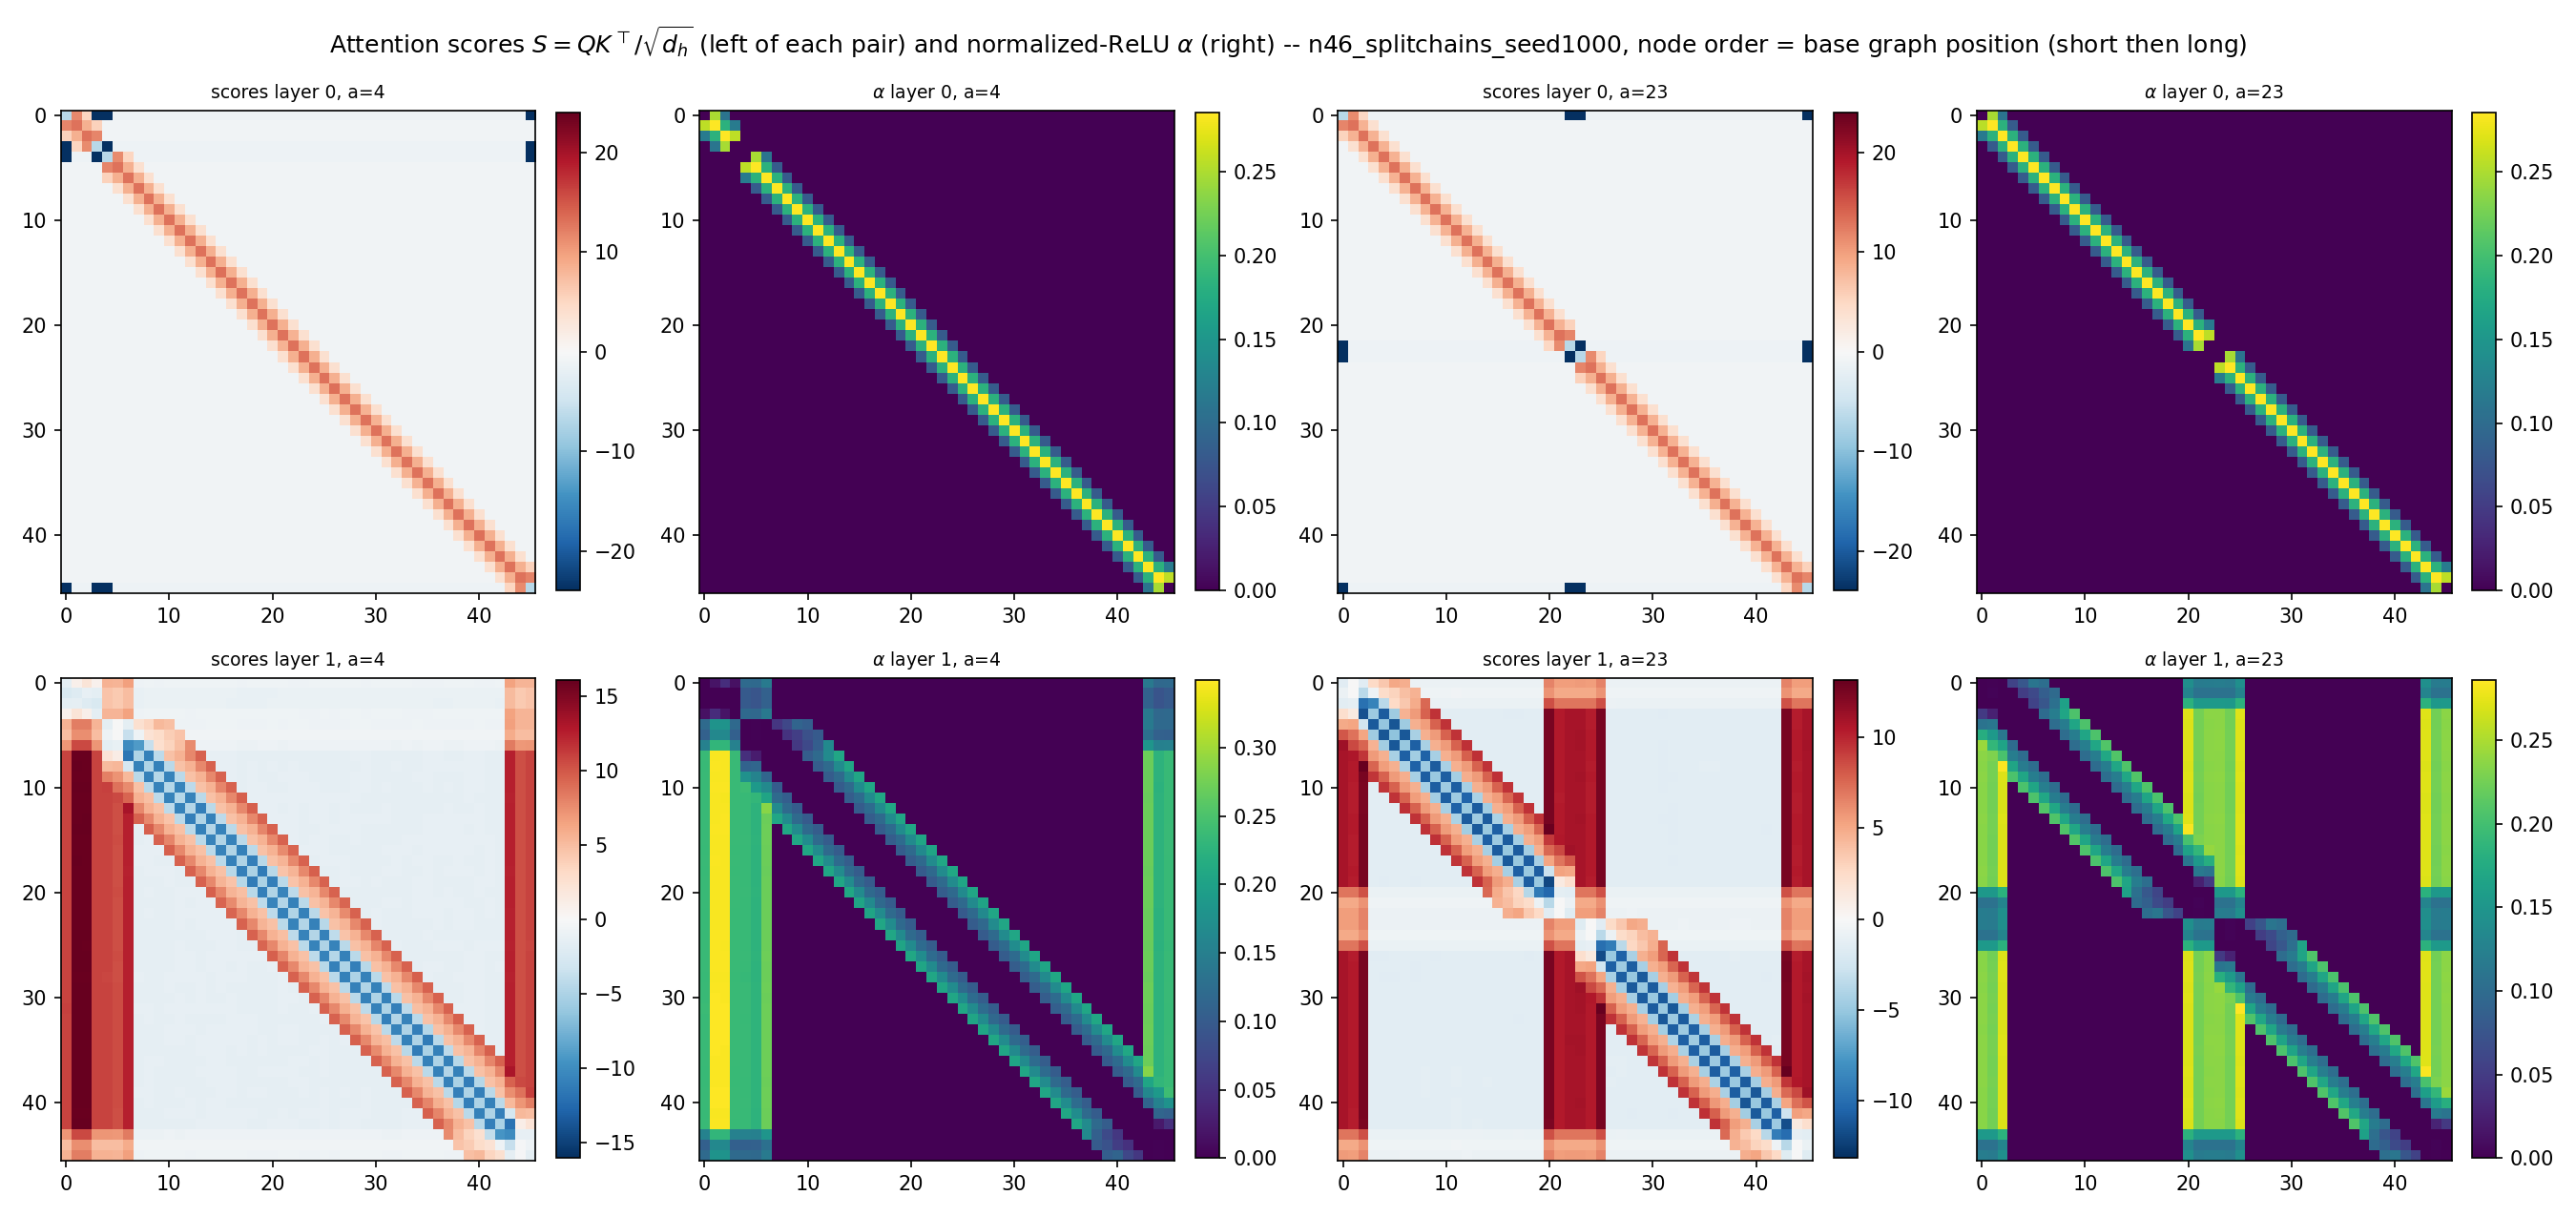
\includegraphics[width=0.95\textwidth]{figs/r9_heatmap_attention_scores_n46_splitchains.png}
\caption{Real attention scores $S$ and normalised-ReLU $\alpha$, layer $0$ (top) / layer $1$
(bottom), $a=4$ and $a=23$, seed $1000$.}
\end{figure}

\begin{figure}[H]\centering
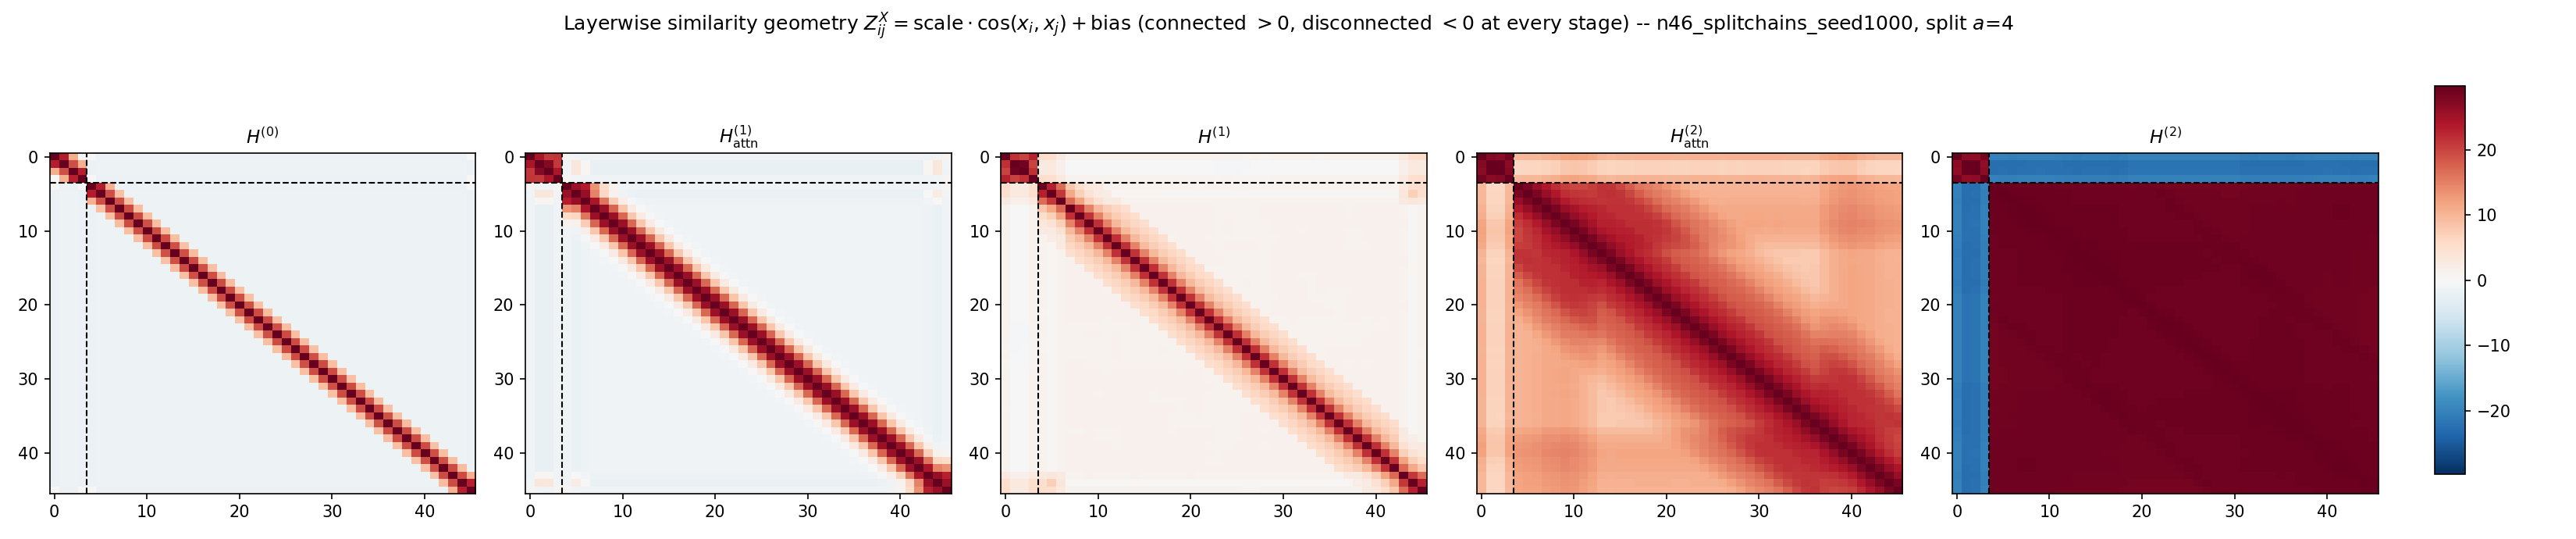
\includegraphics[width=0.95\textwidth]{figs/r9_stagewise_cosine_a4_n46_splitchains.png}
\caption{Five-stage similarity geometry, split $a=4$ (solved, well below the break), seed
$1000$, trained only on random two-chain splits.}
\end{figure}

\begin{figure}[H]\centering
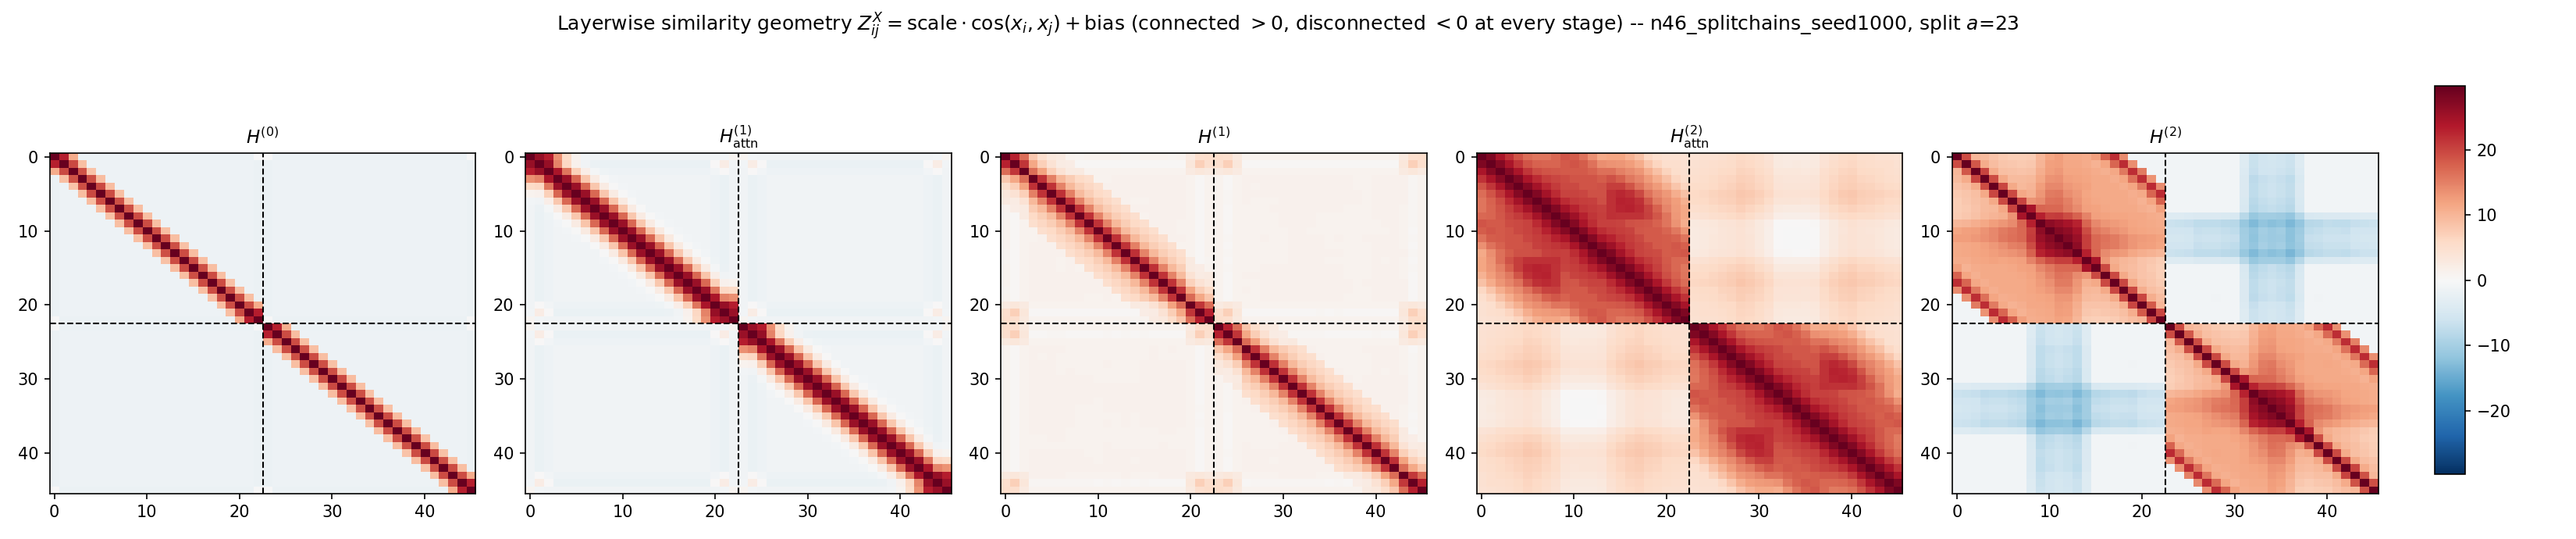
\includegraphics[width=0.95\textwidth]{figs/r9_stagewise_cosine_a23_n46_splitchains.png}
\caption{Five-stage similarity geometry, split $a=23$ (balanced), seed $1000$, trained only on
random two-chain splits.}
\end{figure}

\clearpage
\section{1+2-path training}

\paragraph{Result: essentially identical to 2-chains-only.} Adding the single-chain case
($k{=}1$) to the mixture changes almost nothing: exact match again breaks at exactly $a=12$,
reach(long) again drops to $0.77$ and recovers to $0.92$ by the balanced split, and cut again
stays high throughout ($\ge0.95$ everywhere, only mildly softer than the 2-chains-only
condition's flat $1.000$ at the most balanced splits). The completion signal is robust to which
of the two narrower mixtures is used.

\begin{table}[H]\centering\small
\begin{tabular}{ccccc}
\toprule
$a$ & exact & reach(long) & reach(short) & cut \\
\midrule
1--11 & 1.000 & 1.000 & 1.000 & 1.000 \\
\textbf{12} & \textbf{0.000} & \textbf{0.767} & 1.000 & 1.000 \\
15 & 0.000 & 0.801 & 1.000 & 0.998 \\
18 & 0.000 & 0.845 & 0.989 & 0.997 \\
20 & 0.000 & 0.876 & 0.967 & 0.975 \\
23 & 0.000 & 0.924 & 0.922 & 0.954 \\
\bottomrule
\end{tabular}
\caption{Split sweep $(a,46{-}a)$, seed $1000$ only, trained on a $50/50$ mixture of a single
$46$-node chain and random two-chain splits.}
\end{table}

\begin{figure}[H]\centering
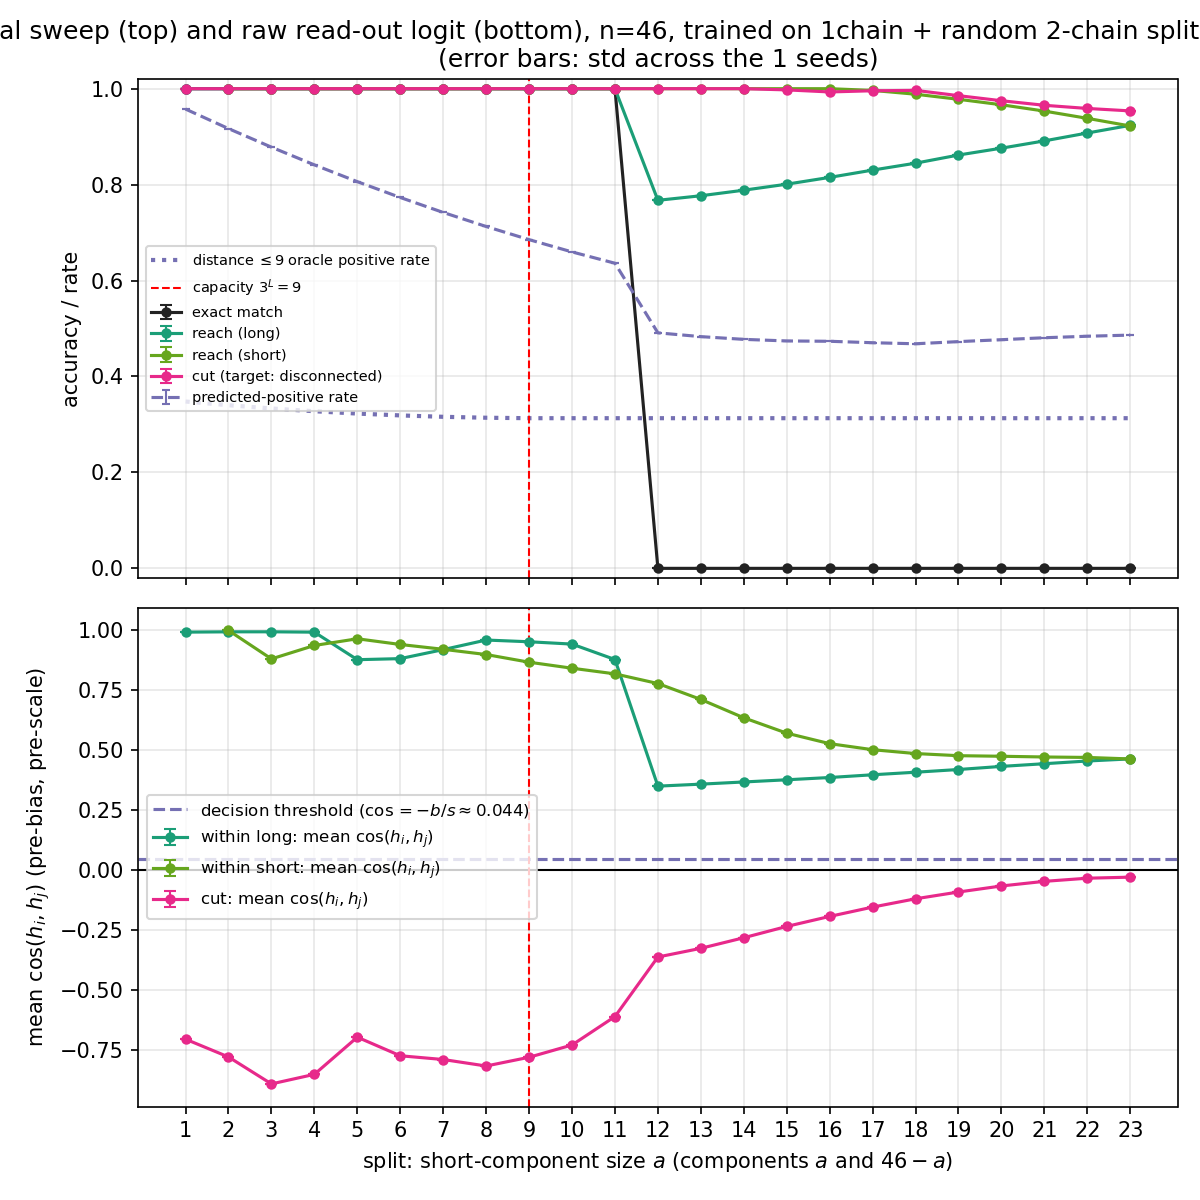
\includegraphics[width=0.95\textwidth]{figs/r9_sweep_and_logit_n46_onetwopath.png}
\caption{Full sweep + raw similarity logit, seed $1000$, trained on 1chain+split\_chains.}
\end{figure}

\begin{figure}[H]\centering
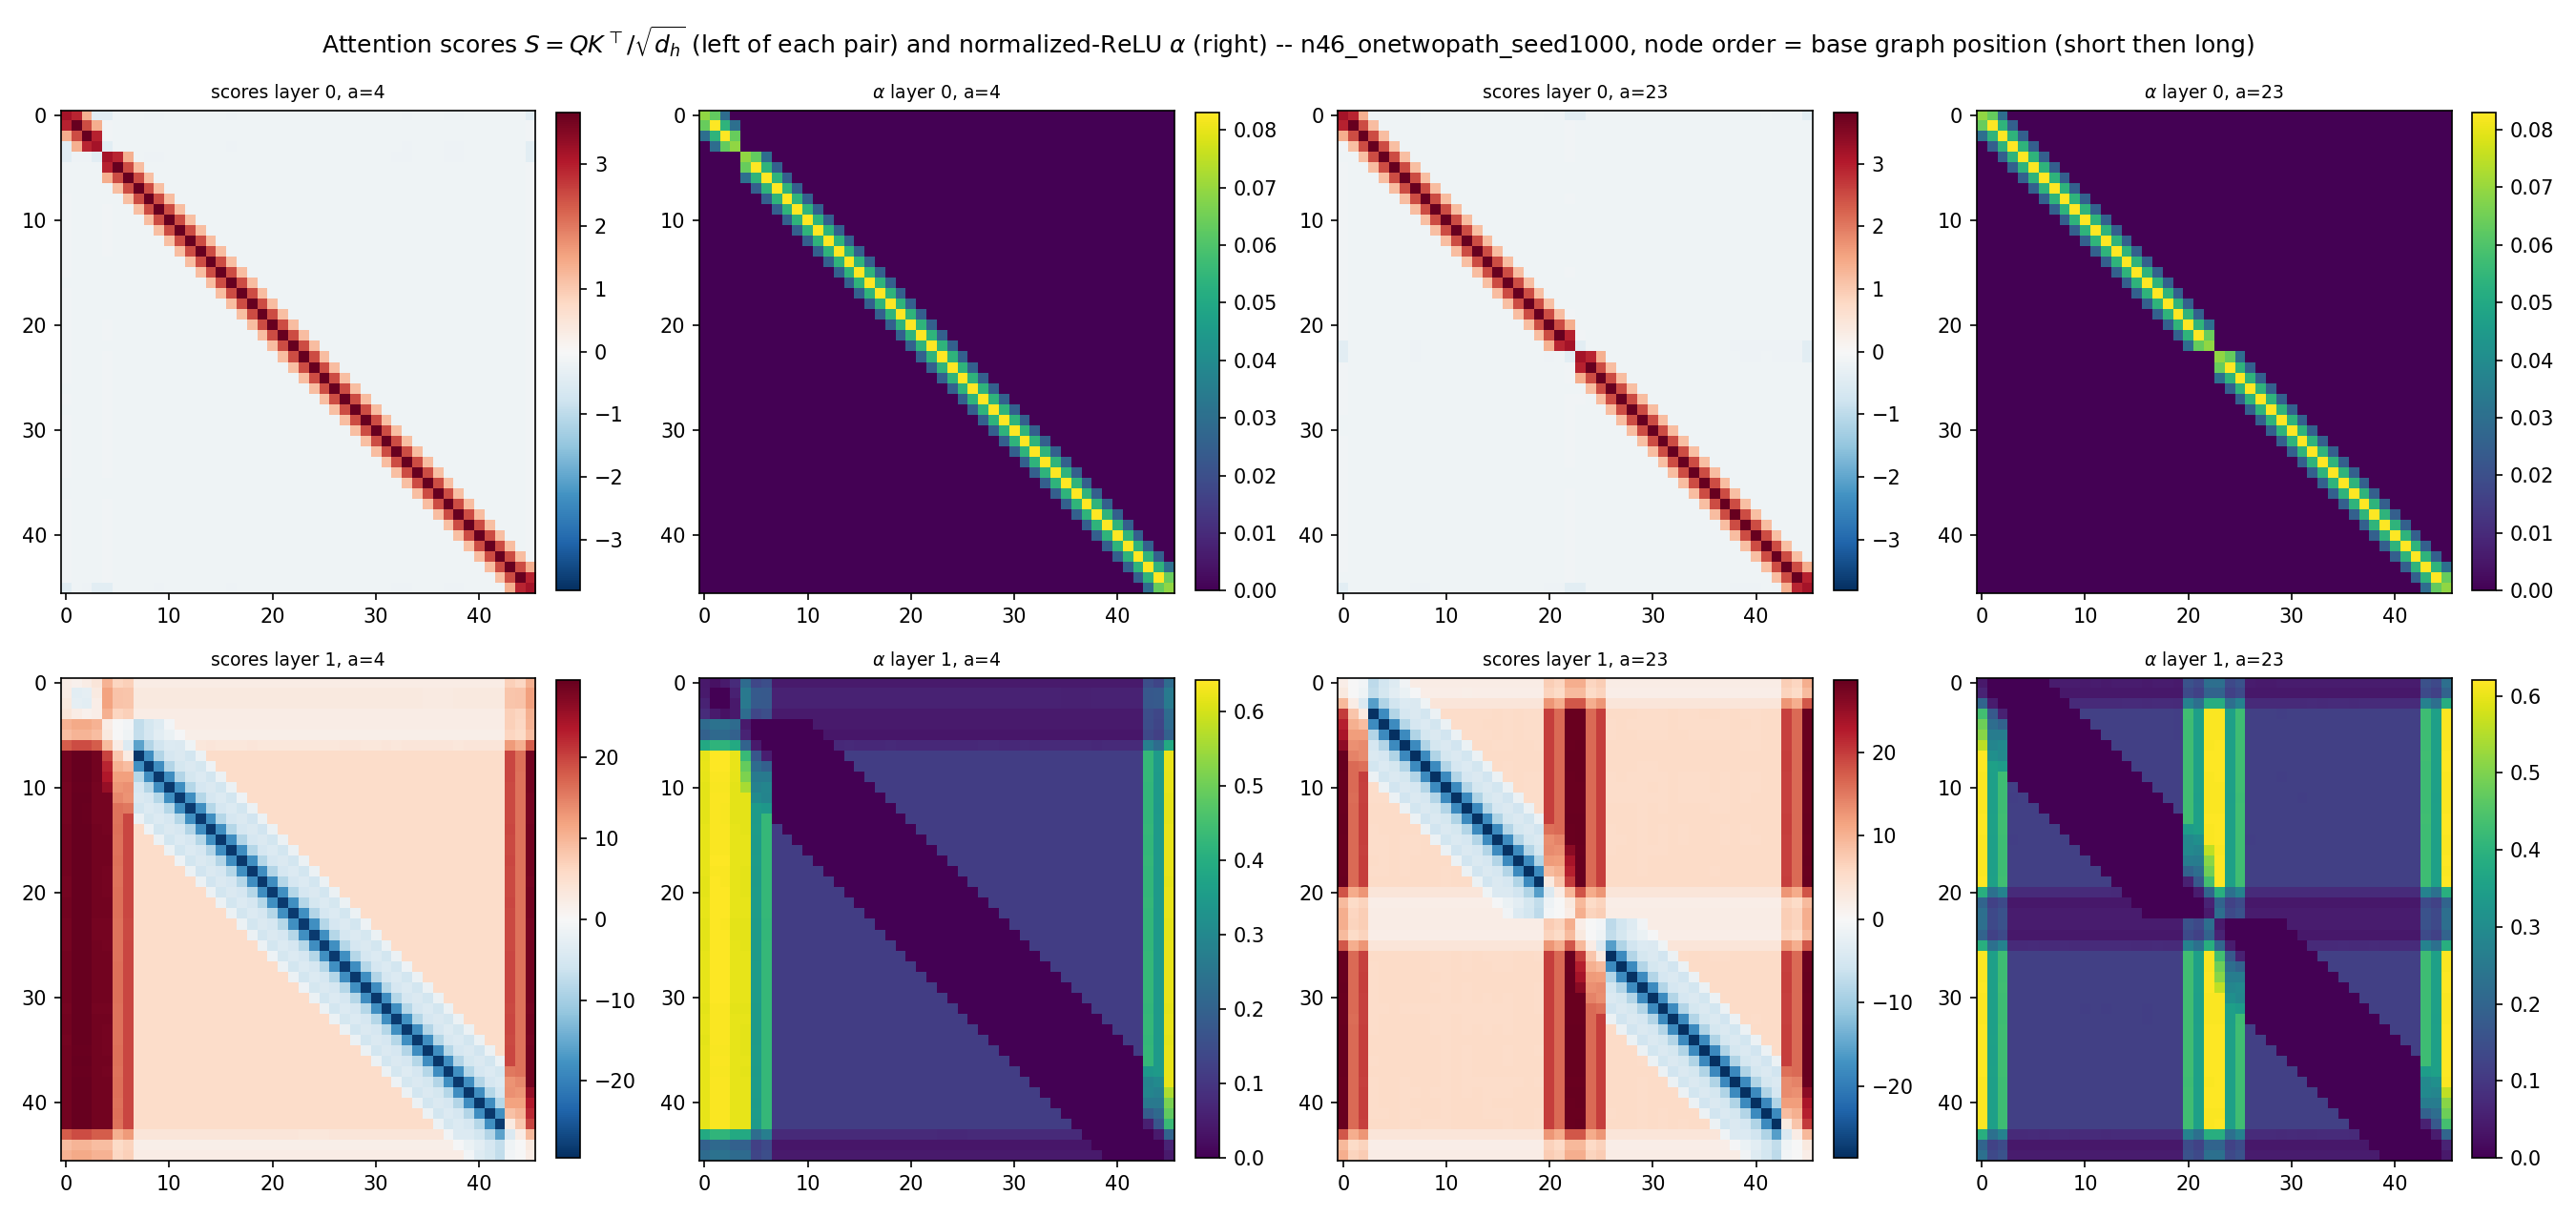
\includegraphics[width=0.95\textwidth]{figs/r9_heatmap_attention_scores_n46_onetwopath.png}
\caption{Real attention scores $S$ and normalised-ReLU $\alpha$, layer $0$ (top) / layer $1$
(bottom), $a=4$ and $a=23$, seed $1000$.}
\end{figure}

\begin{figure}[H]\centering
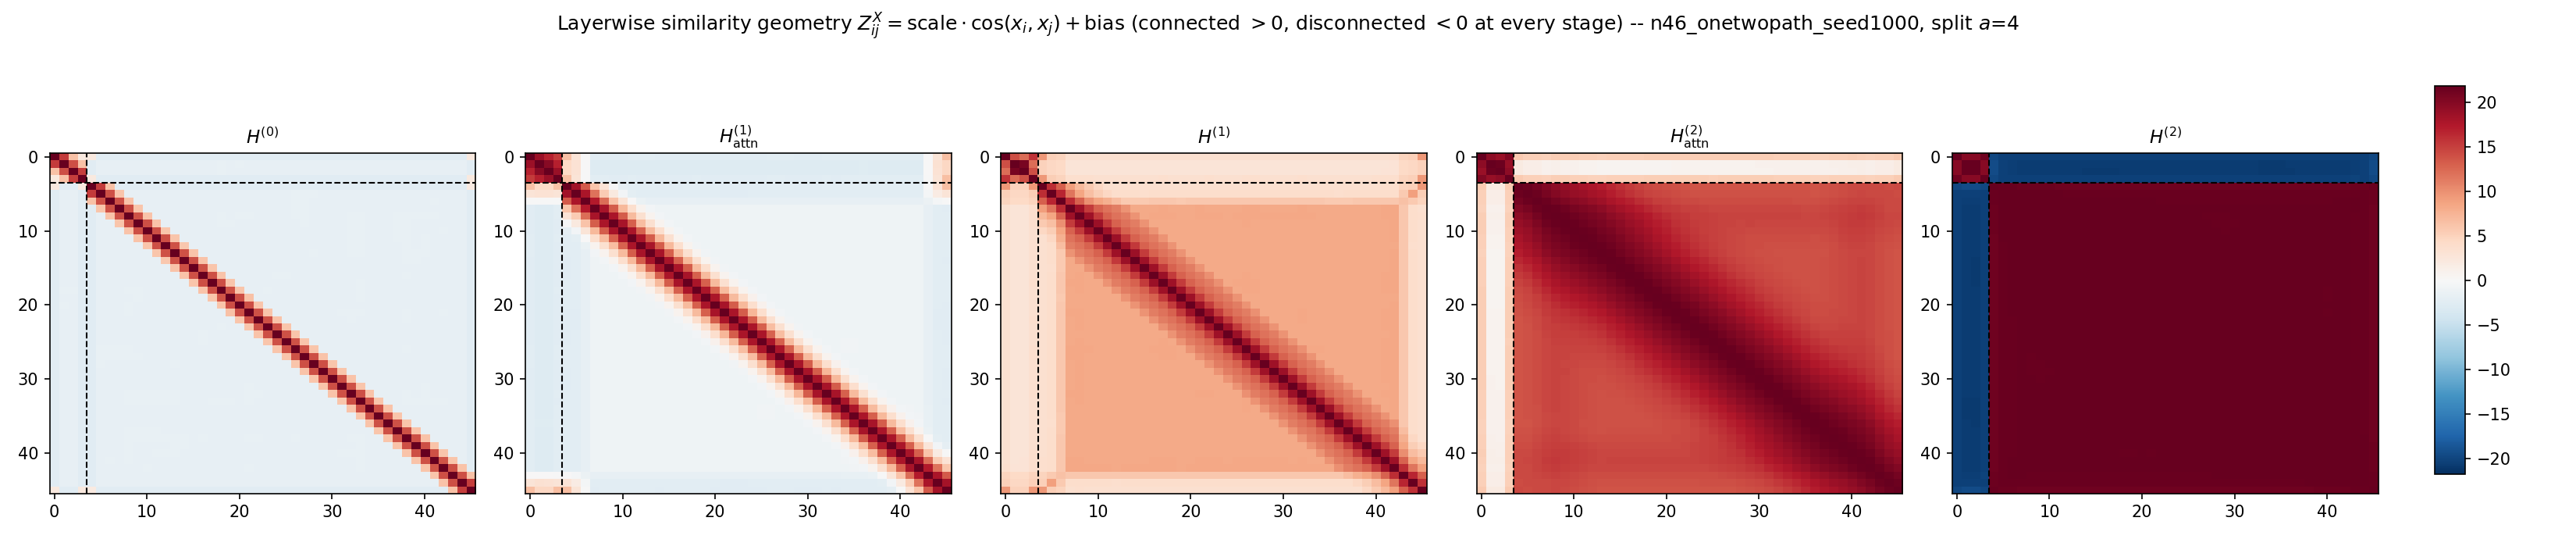
\includegraphics[width=0.95\textwidth]{figs/r9_stagewise_cosine_a4_n46_onetwopath.png}
\caption{Five-stage similarity geometry, split $a=4$ (solved, well below the break), seed
$1000$, trained on 1chain+split\_chains.}
\end{figure}

\begin{figure}[H]\centering
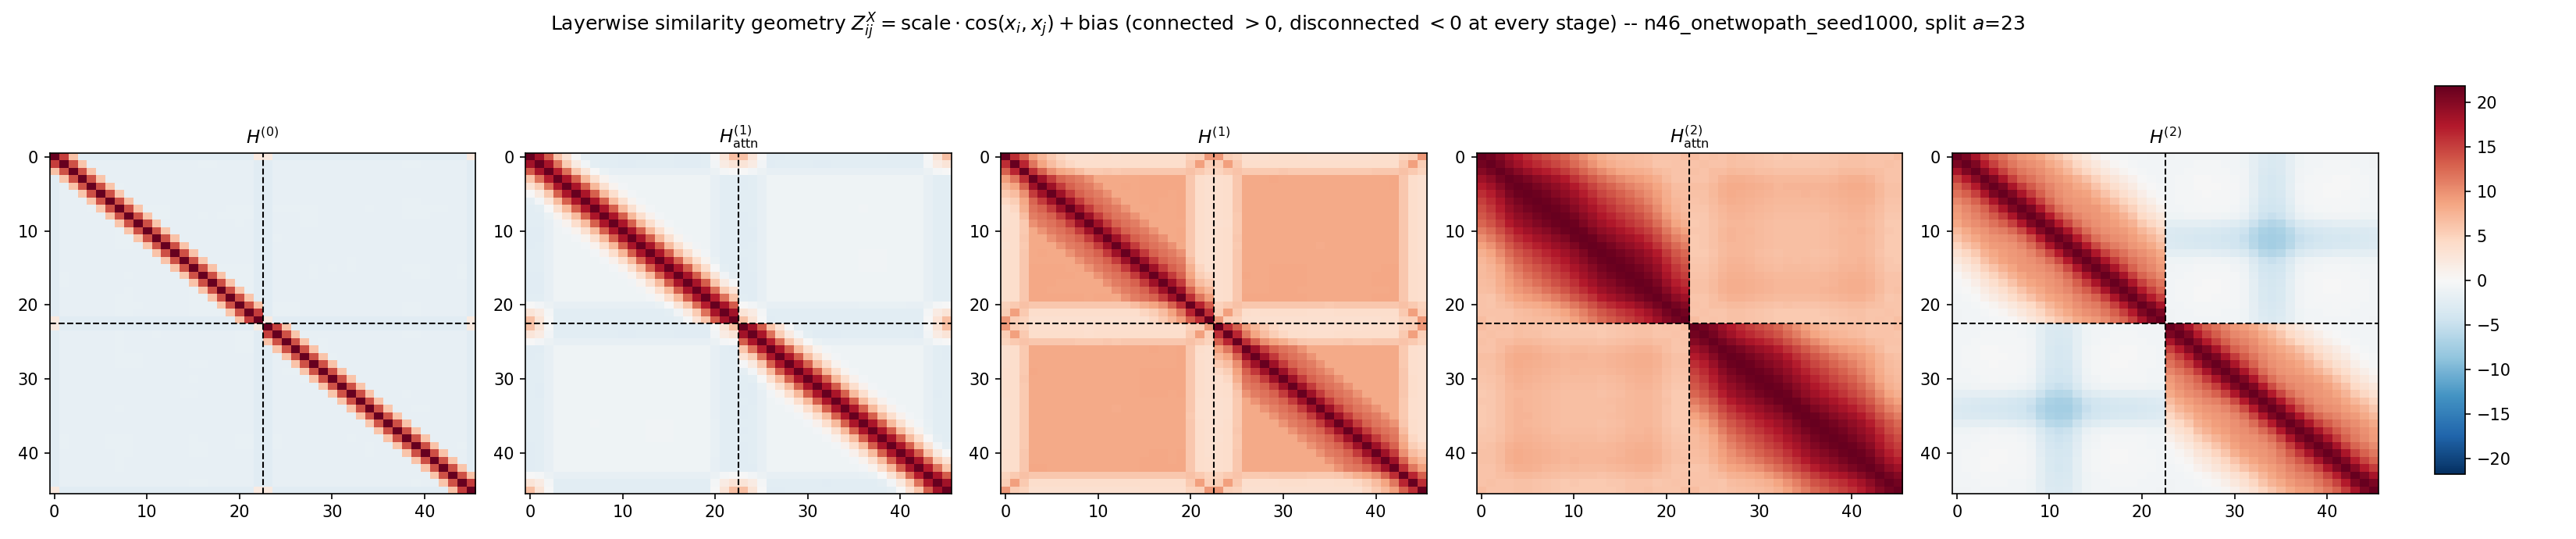
\includegraphics[width=0.95\textwidth]{figs/r9_stagewise_cosine_a23_n46_onetwopath.png}
\caption{Five-stage similarity geometry, split $a=23$ (balanced), seed $1000$, trained on
1chain+split\_chains.}
\end{figure}

\clearpage
\section{2-cycles-only training --- a genuinely different failure mode}

\paragraph{Result: reach stays perfect everywhere; cut collapses totally and sharply, unlike
every chain-based condition.} Trained \emph{specifically and systematically} on two-cycle splits
(removing Report~VIII's ``never seen a cycle at all'' confound entirely), the model shows a
strikingly different signature from every chain-based condition above:

\begin{itemize}\setlength\itemsep{0.1em}
  \item Reach inside both components is \emph{exactly} $1.000$ at \emph{every} split tested,
        $a=6$ through $a=23$ -- no dip at the break point at all, unlike every chain condition
        (which all show a $\sim0.2$ dip in reach(long) right at the break).
  \item Cut is $\ge0.94$ for $a\le11$, then collapses to \emph{exactly} $0.000$ at $a=12$ and
        stays \emph{exactly} $0.000$ all the way to the balanced split $a=23$ -- not a gradual
        softening like the chain conditions, a complete, permanent switch to calling every
        cross-cycle pair connected.
  \item One honest caveat: the smallest splits ($a=3,4,5$) are noisy (exact $0.78, 0.51, 0.375$)
        before the sweep stabilises to $1.000$ at $a=6$--$11$ -- a single seed, so this could be
        sampling noise around an unusually small/degenerate cycle size, not necessarily a real
        effect; not investigated further here.
\end{itemize}

\begin{table}[H]\centering\small
\begin{tabular}{cccccc}
\toprule
$a$ & exact & reach(long) & reach(short) & cut & pred.\ positive rate \\
\midrule
3 & 0.780 & 1.000 & 1.000 & 0.985 & 0.880 \\
4 & 0.510 & 1.000 & 1.000 & 0.938 & 0.851 \\
5 & 0.375 & 1.000 & 1.000 & 0.911 & 0.824 \\
6--11 (avg) & 1.000 & 1.000 & 1.000 & 1.000 & 0.701 \\
\textbf{12} & \textbf{0.000} & \textbf{1.000} & \textbf{1.000} & \textbf{0.000} & \textbf{1.000} \\
15 & 0.000 & 1.000 & 1.000 & 0.000 & 1.000 \\
18 & 0.000 & 1.000 & 1.000 & 0.000 & 1.000 \\
23 & 0.000 & 1.000 & 1.000 & 0.000 & 1.000 \\
\bottomrule
\end{tabular}
\caption{Split sweep $(a,46{-}a)$, seed $1000$ only, trained ONLY on random two-cycle splits
(each segment closed into a ring). Note reach is always exact; cut drops to exactly $0$, not a
soft floor. \textbf{The predicted-positive rate is EXACTLY $1.000$ from $a=12$ onward}: past
the break, the model predicts every single pair in the graph (all $n^2$ of them, not just the
cross pairs) as ``connected'' -- not a selective cut failure, but total collapse to ``yes''.
Since within-component pairs are trivially correctly ``connected'' regardless, a 2-component
graph alone cannot tell this apart from the model having learned to selectively recognise the
small component and correctly separate it -- a 3-cycle test (pending, see below once the job
returns) is needed for a graph that CAN tell the two apart.}
\end{table}

\begin{figure}[H]\centering
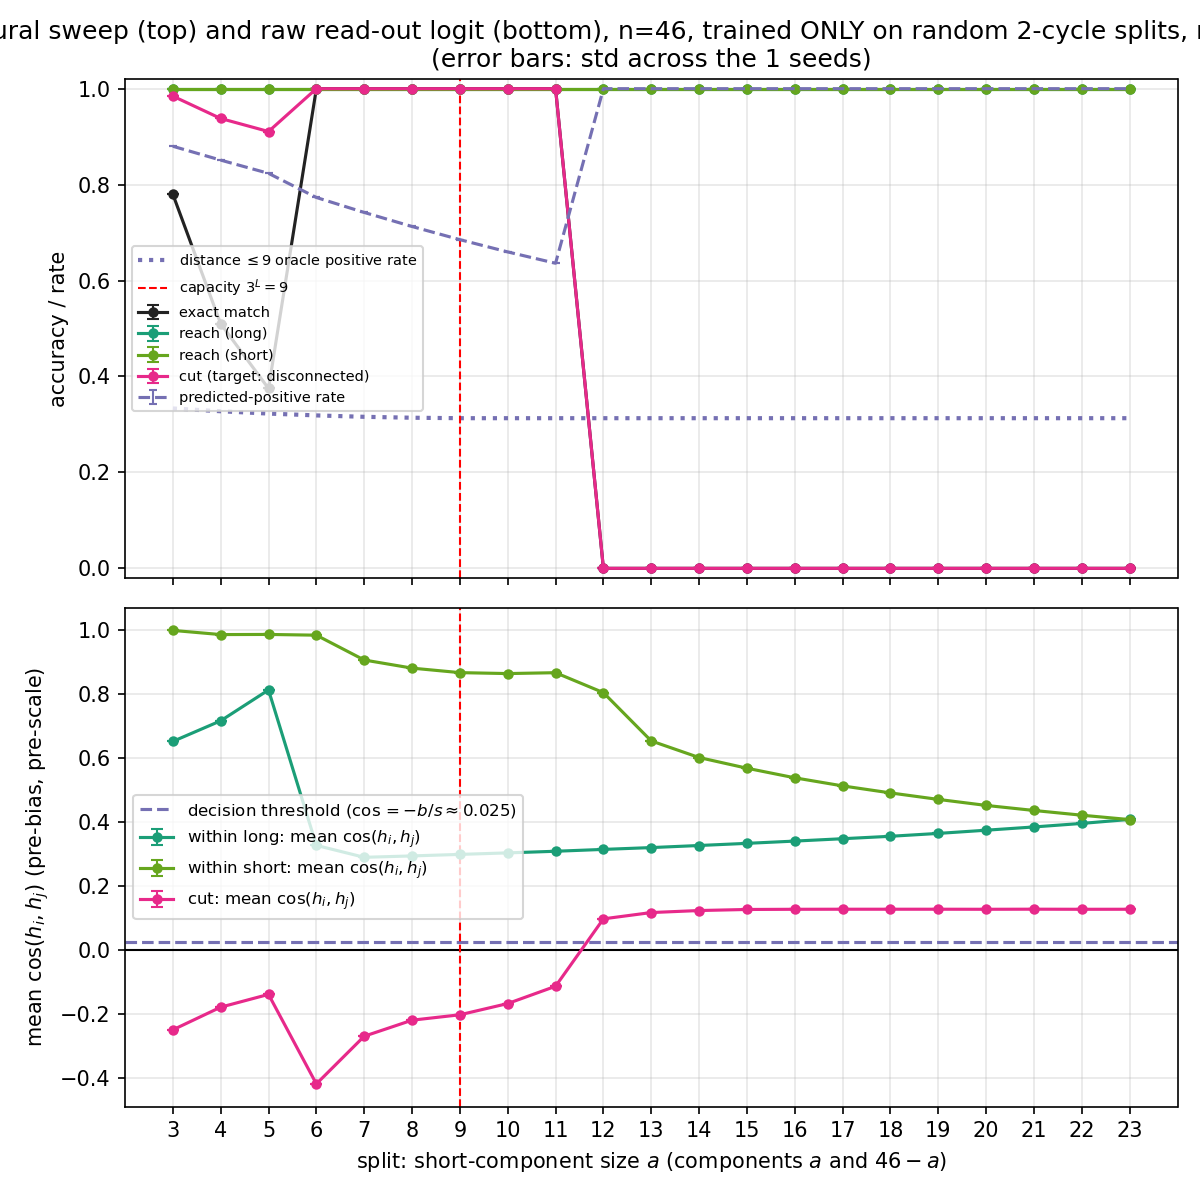
\includegraphics[width=0.95\textwidth]{figs/r9_sweep_and_logit_n46_splitcycles.png}
\caption{Full sweep + raw similarity logit, seed $1000$, trained only on random two-cycle
splits. Note the cut curve (pink) hits exactly $0$ at $a=12$ and never recovers, unlike the
gradual softening in the two chain-based conditions above.}
\end{figure}

\begin{figure}[H]\centering
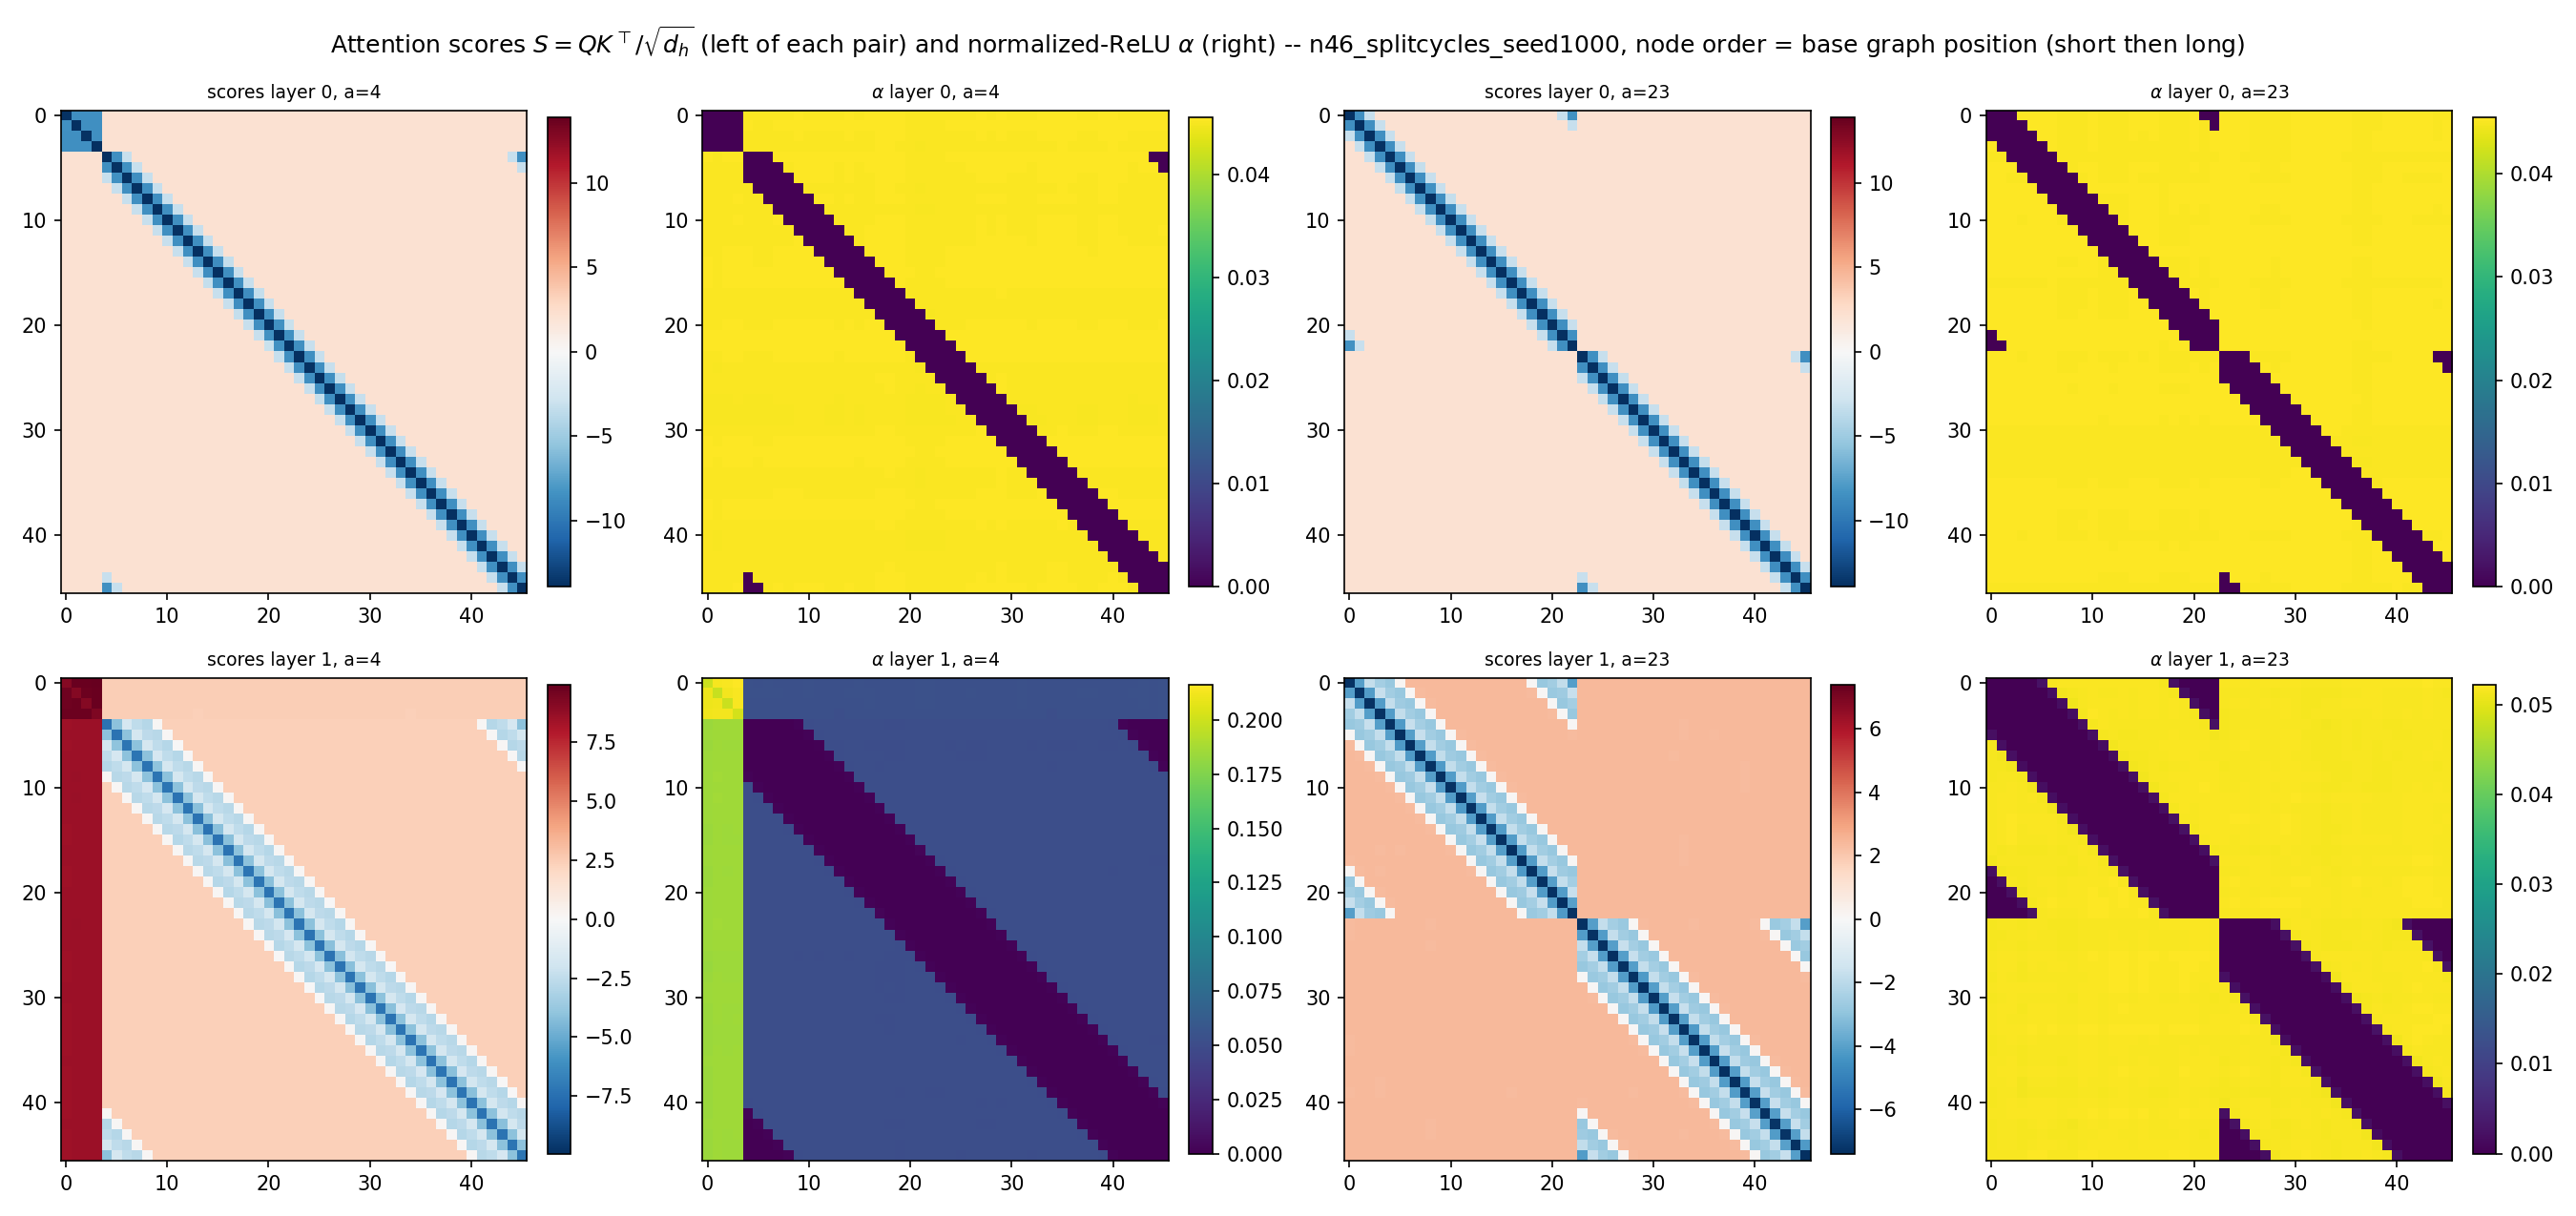
\includegraphics[width=0.95\textwidth]{figs/r9_heatmap_attention_scores_n46_splitcycles.png}
\caption{Real attention scores $S$ and normalised-ReLU $\alpha$, layer $0$ (top) / layer $1$
(bottom), $a=4$ and $a=23$, seed $1000$. Layer $1$ $\alpha$ is far more uniformly high across
almost the entire matrix at $a=23$ than in either chain-based condition, where the high-$\alpha$
region was concentrated in bands connecting specific components rather than nearly everywhere.}
\end{figure}

\begin{figure}[H]\centering
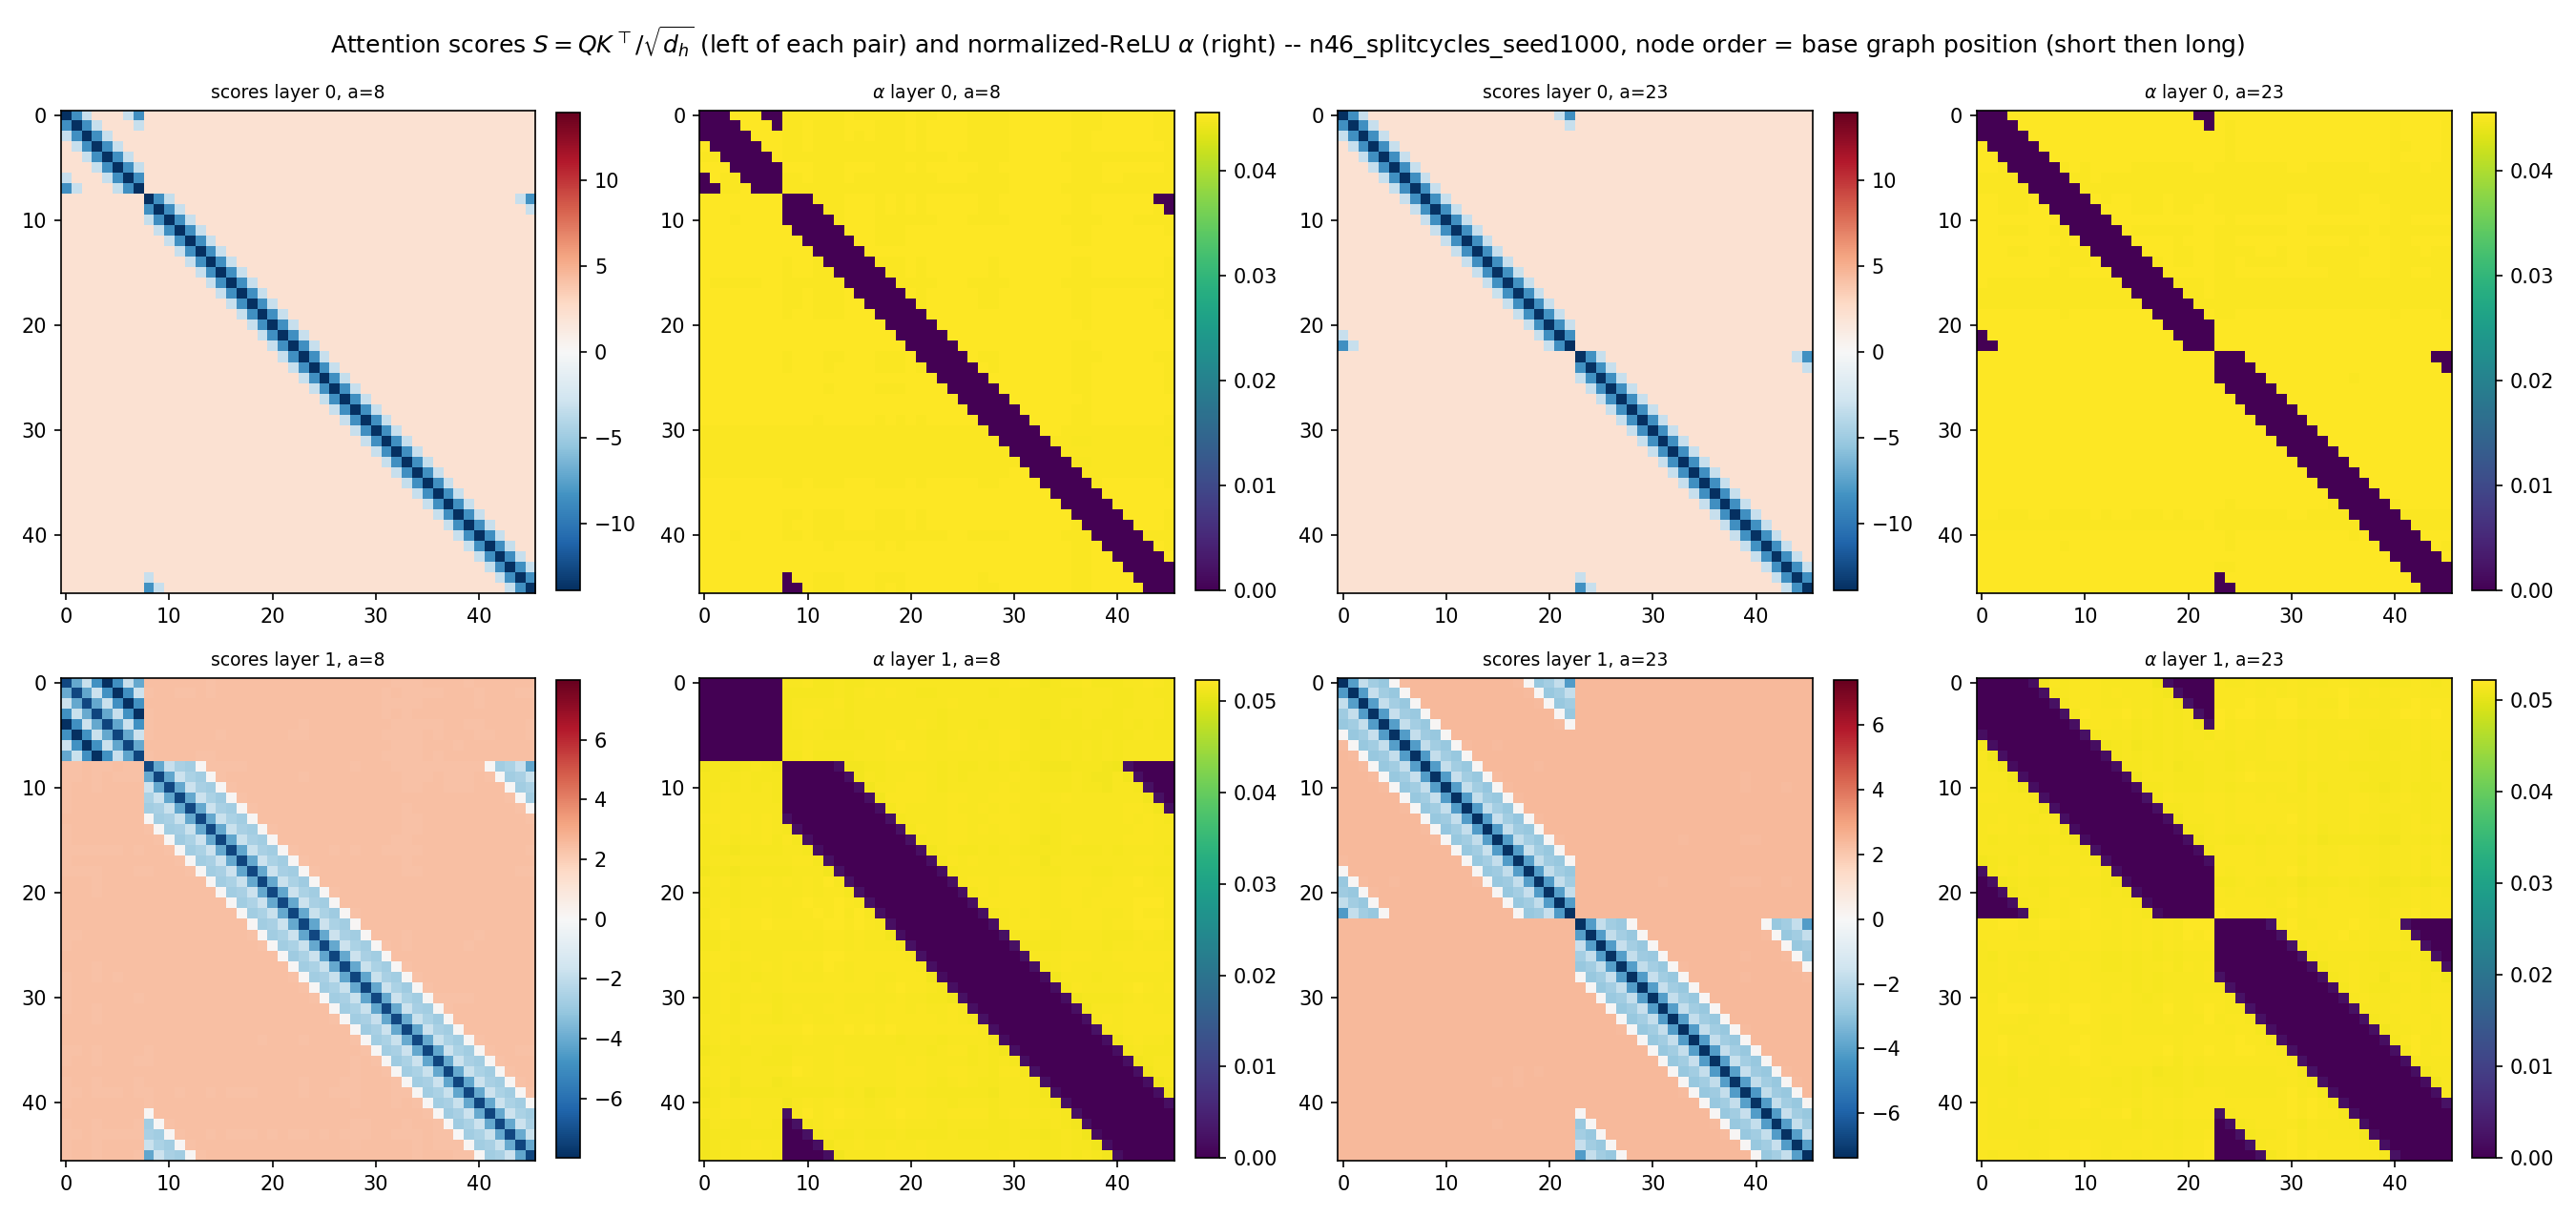
\includegraphics[width=0.95\textwidth]{figs/r9_heatmap_attention_scores_n46_splitcycles_a8.png}
\caption{Same, but $a=8$ vs $a=23$ -- $a=8$ is a more honest ``solved'' reference point than
$a=4$ above, since it sits inside the clean $a=6$--$11$ plateau (exact match $=1.000$) rather
than the borderline $a=4$ cell (exact match only $0.51$).}
\end{figure}

\begin{figure}[H]\centering
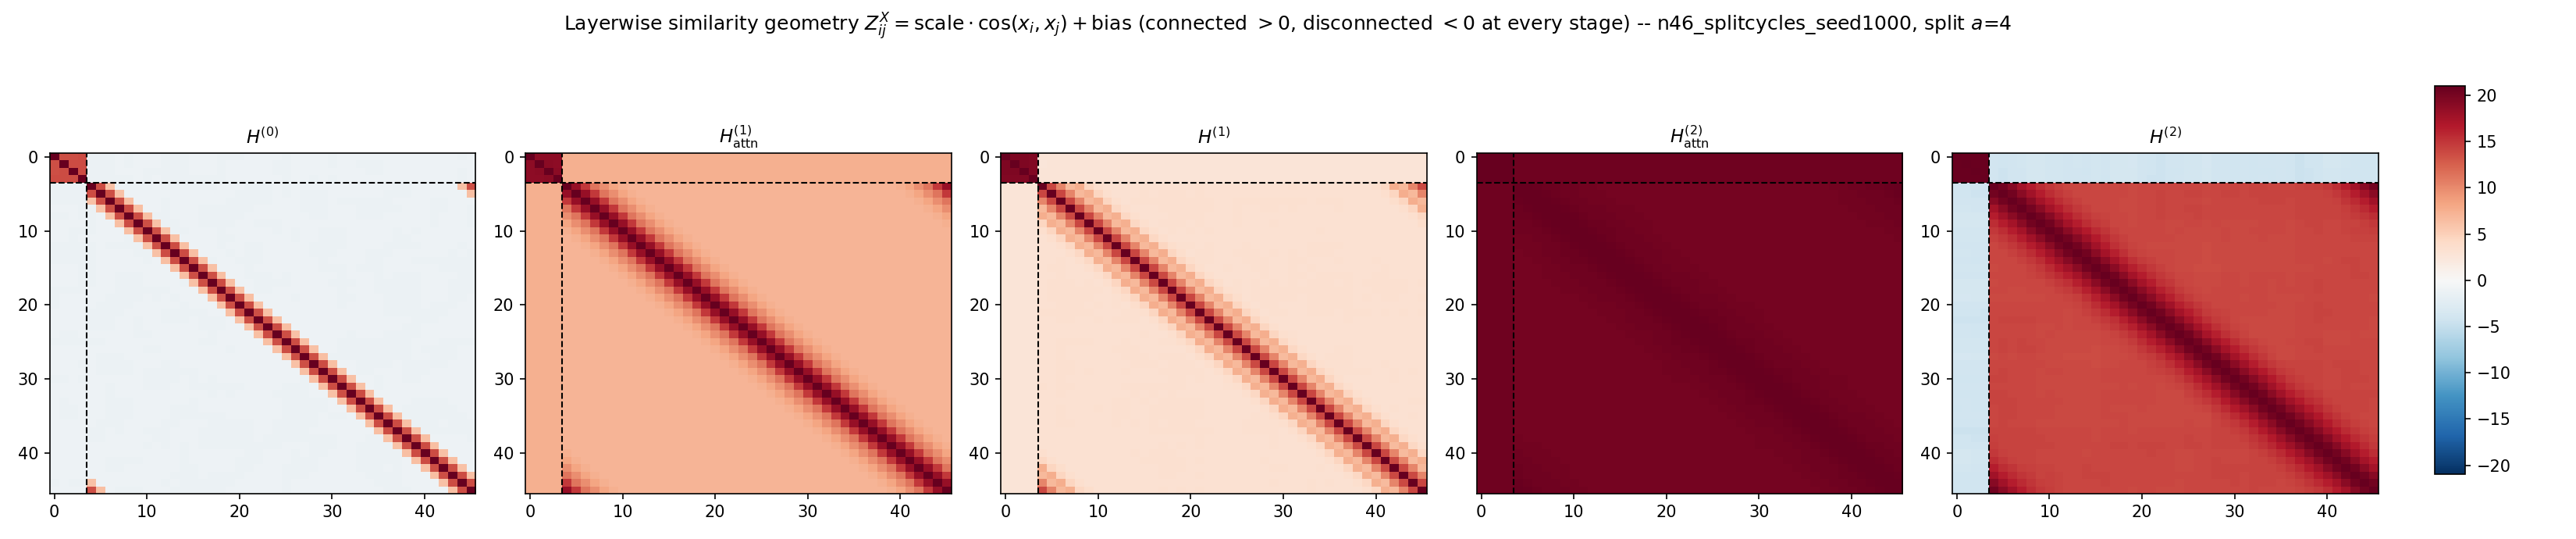
\includegraphics[width=0.95\textwidth]{figs/r9_stagewise_cosine_a4_n46_splitcycles.png}
\caption{Five-stage similarity geometry, split $a=4$ (borderline, exact $=0.51$), seed $1000$.}
\end{figure}

\begin{figure}[H]\centering
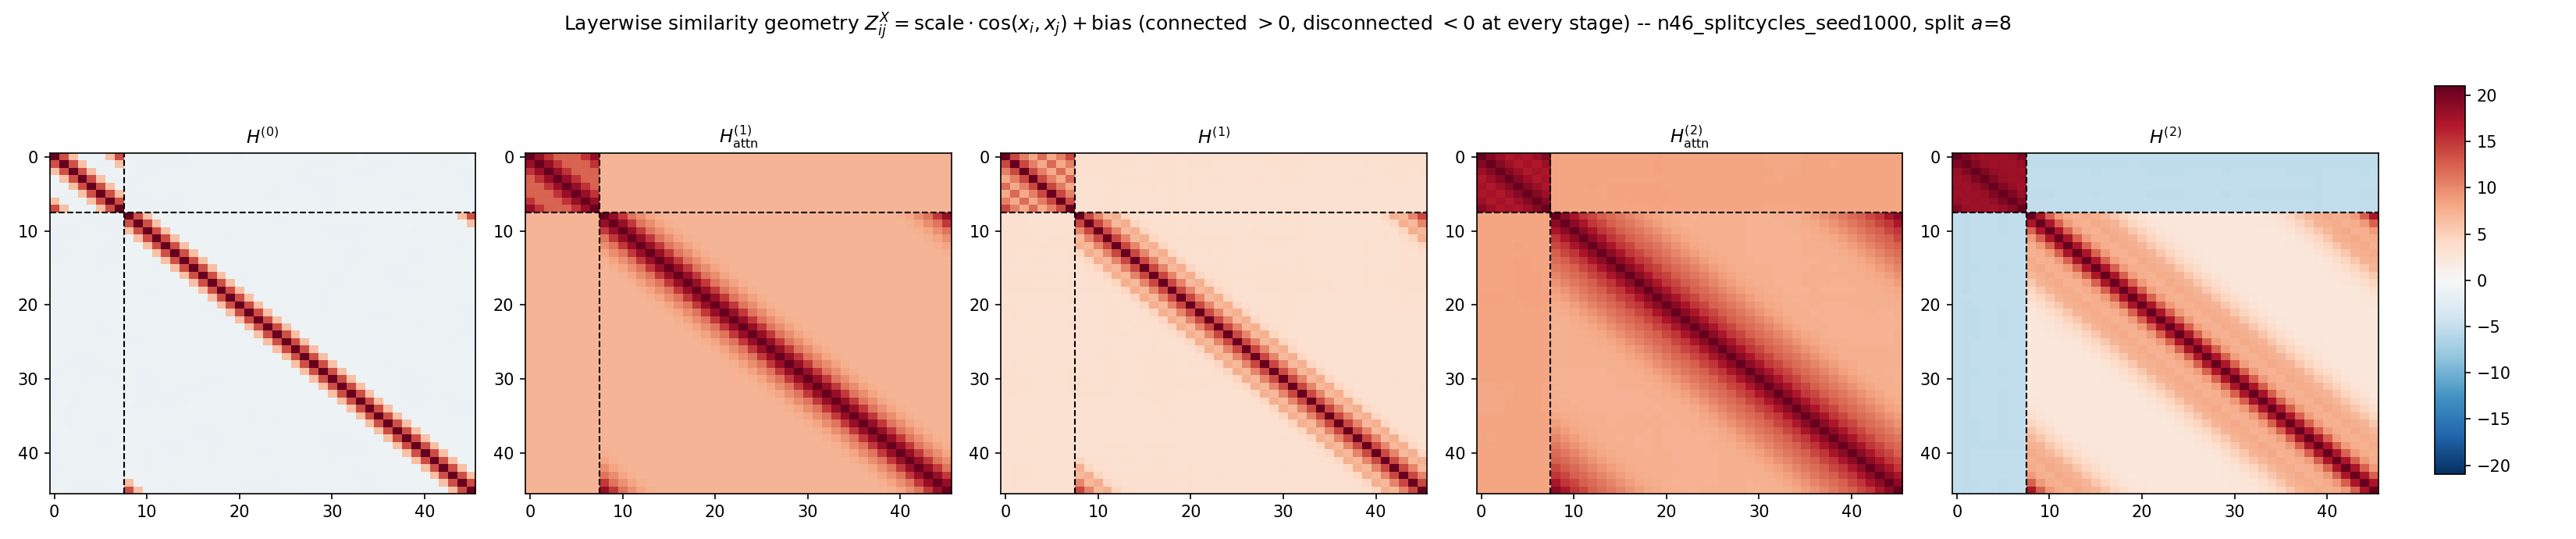
\includegraphics[width=0.95\textwidth]{figs/r9_stagewise_cosine_a8_n46_splitcycles.png}
\caption{Five-stage similarity geometry, split $a=8$ (cleanly solved, exact $=1.000$, inside the
$a=6$--$11$ plateau), seed $1000$ -- the more honest ``before the break'' reference point.}
\end{figure}

\begin{figure}[H]\centering
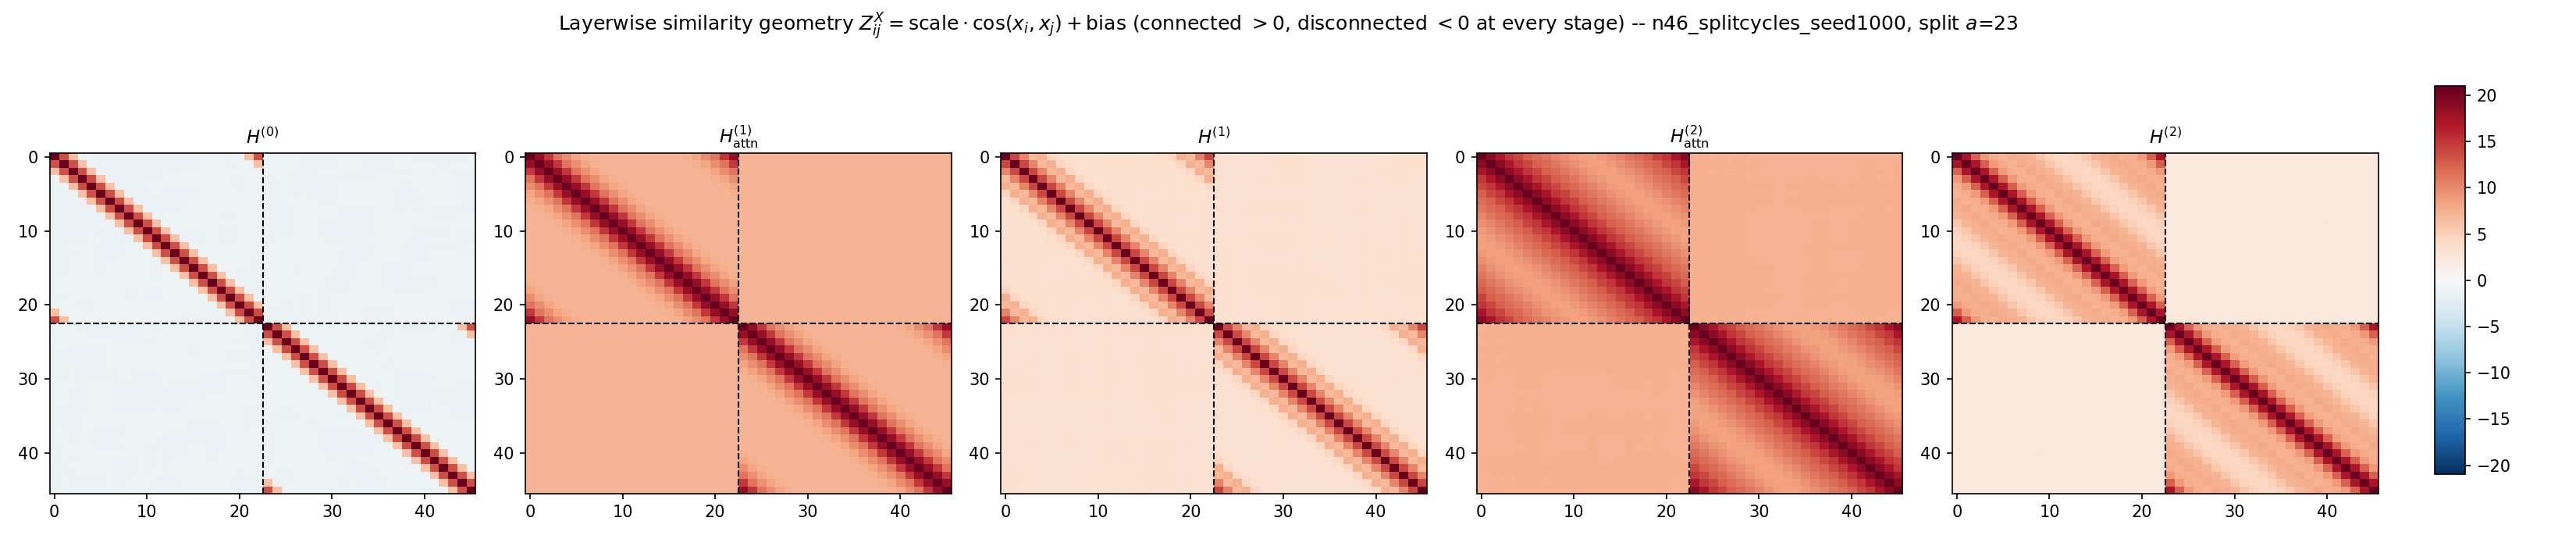
\includegraphics[width=0.95\textwidth]{figs/r9_stagewise_cosine_a23_n46_splitcycles.png}
\caption{Five-stage similarity geometry, split $a=23$ (balanced, totally failed), seed $1000$.
Note the cross-component block is already mildly \emph{positive} (pale red, not blue) at
$H^{(0)}$ -- before any attention runs at all -- and never turns negative at any later stage,
unlike the chain-based conditions where the cross block starts clearly negative at $H^{(0)}$.}
\end{figure}

\paragraph{A candidate mechanistic reading (tentative, one seed, one representative split).} In
the balanced-split heatmap above, the cross-component block is already faintly on the
``connected'' side of zero at the very first stage $H^{(0)}$ (the read-in embedding, before any
attention or feed-forward computation) and stays that way through every later stage --- it never
crosses into clearly negative territory the way it does for the chain-based conditions. Since
$H^{(0)}$ is built purely from each node's own row of the adjacency matrix, and every node on a
cycle has an \emph{identical} local neighbourhood shape (degree exactly $2$, no distinguished
end), this is consistent with the read-in step itself failing to give cycle nodes from different
components a distinguishing signature the way a path's endpoint-distance does for chain nodes ---
before the network has any chance to build a genuine cut decision downstream. This is offered as a
candidate explanation to test further (e.g.\ by looking at $H^{(0)}$ across more splits and
seeds), not a settled conclusion.

\clearpage
\section{Thread A.3: does the split\_chains-only checkpoint survive a genuine third
component? All 176 size combinations}

The 2-chains-only checkpoint from \S1 was trained EXCLUSIVELY on graphs with exactly 2 disjoint
path components, never 3 or more -- so a genuine three-component graph is out-of-distribution in
component \emph{count} for this checkpoint specifically (unlike the three-component tests of
Reports~VII/VIII, whose training streams already covered 3--4 components). This is the direct
implementation of Thread~A.3 of the plan: take the same two-way split and remove one internal
edge from one of the two paths, producing 3 disjoint paths with sizes the training stream could
never have produced. Every distinct combination of resulting sizes was tested -- every partition
of $n=46$ into 3 positive parts $(s_1\le s_2\le s_3)$, $176$ cells in total, $200$ random
relabellings per cell -- purely behavioural for now (exact match, reach inside each component,
cut between each of the three pairs); no attention scores or layerwise geometry yet, pending a
choice of which specific cells are worth the deeper dive.

\paragraph{Headline 1: whole-graph exact match is $0.000$ in every single one of the $176$
cells.} Introducing a genuine third component breaks perfect exact-match completely, with no
exceptions -- even the easiest-looking configurations (e.g.\ a trivial isolated node plus a
short path plus a long one) never get every pair in the graph right simultaneously.

\paragraph{Headline 2: reach stays essentially perfect everywhere; the whole story is which ONE
of the three pairwise cuts fails.} Reach inside each individual component is $\ge0.95$ in nearly
every cell regardless of size (not tabulated in full here since it is uniformly high) -- the
model still resolves distance correctly \emph{inside} each component even with a foreign third
component present. What fails is entirely at the cut level, and remarkably it is usually not a
generic ``confused everywhere'' failure: in most cells exactly ONE of the three pairwise
relationships (comp$_1$-comp$_2$, comp$_1$-comp$_3$, comp$_2$-comp$_3$) is called ``connected''
almost always, while the other two are correctly called ``disconnected'' almost always.

\begin{figure}[H]\centering
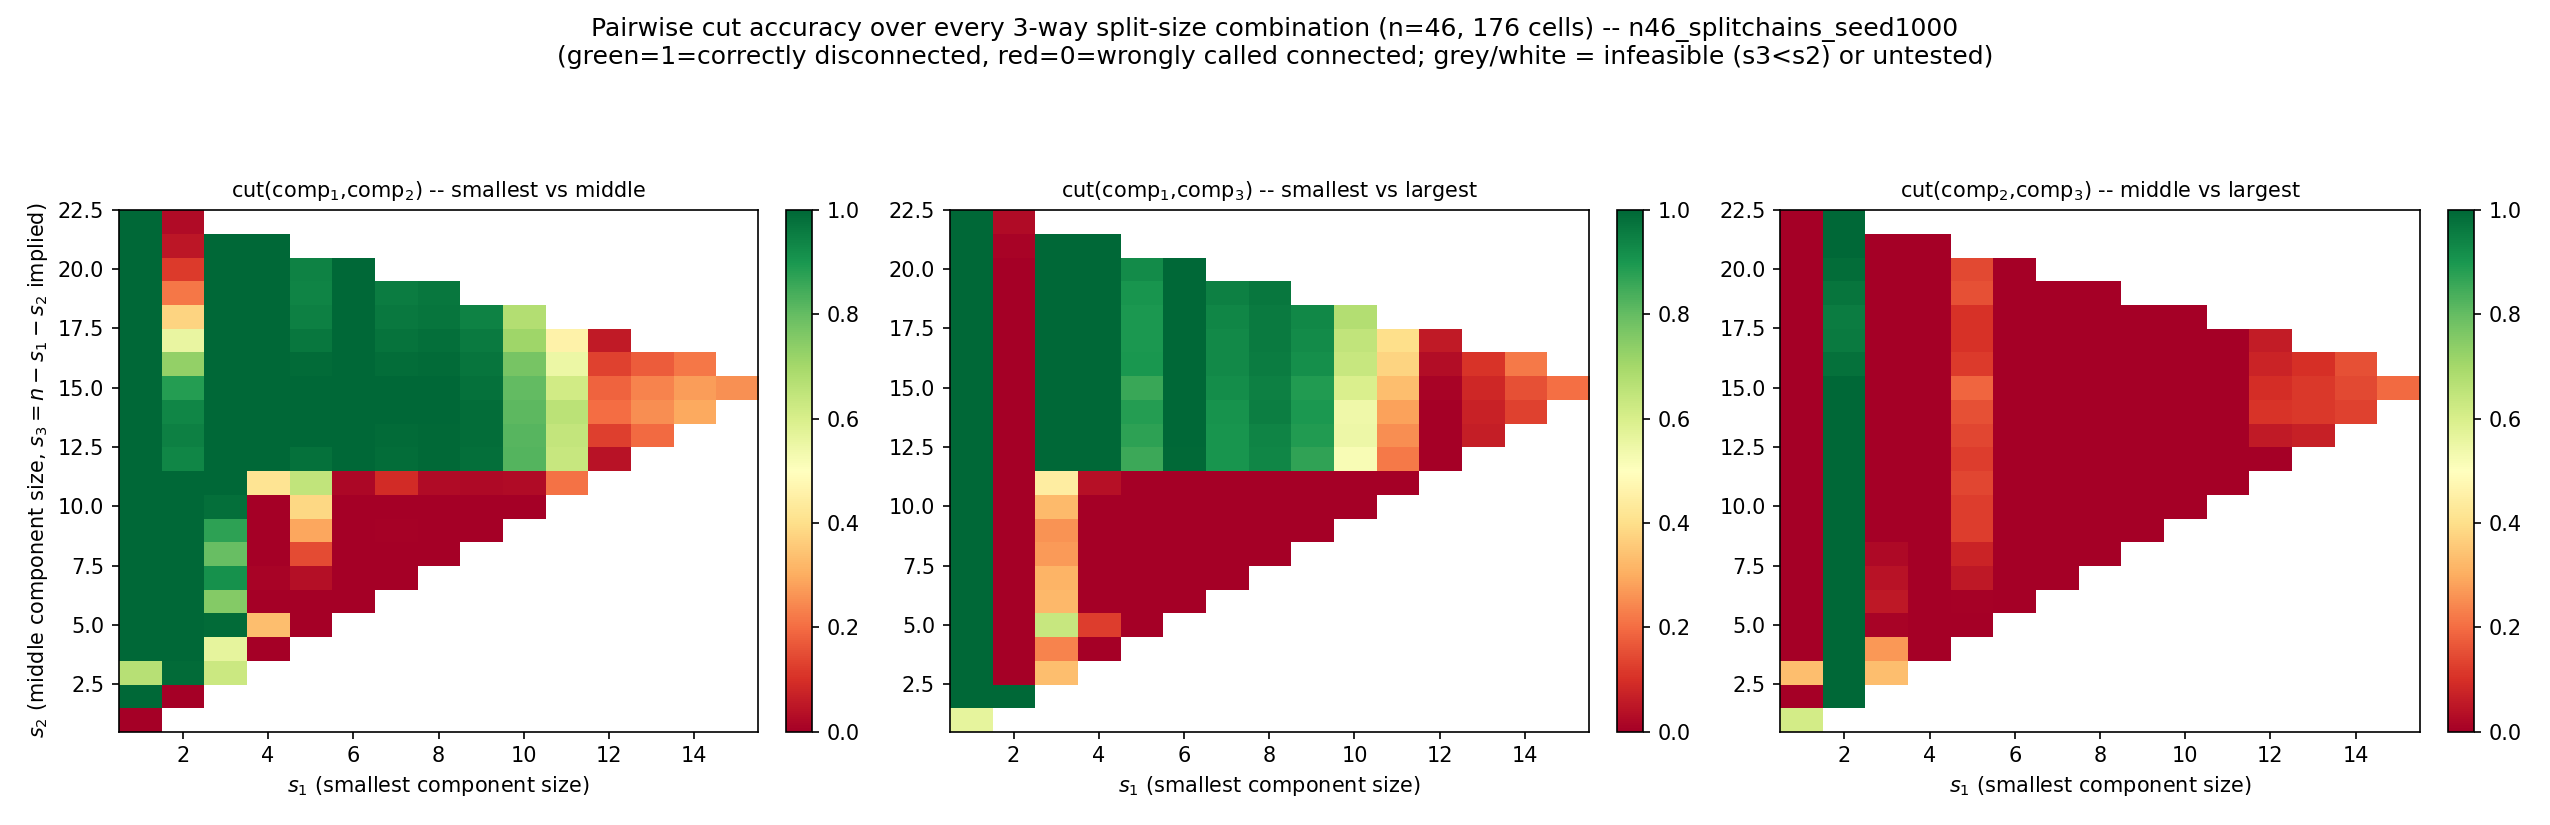
\includegraphics[width=0.98\textwidth]{figs/r9_threeway_cut_heatmaps_n46_splitchains_seed1000.png}
\caption{Each of the three pairwise cut accuracies, over every feasible $(s_1,s_2)$ combination
($s_3=46-s_1-s_2$ implied), green=correctly disconnected, red=wrongly called connected.}
\end{figure}

\paragraph{Headline 3: a component of exactly $1$ node (an isolated node, the training
distribution's own ``short'' extreme) is the ONLY size that lets the model tell the other two
components apart from each other.} The rightmost panel above (cut between the middle and
largest component) is red -- failed -- across almost the \emph{entire} grid, with one striking
exception: a clean green vertical stripe at $s_1=1$. The moment the smallest component has any
internal structure at all ($s_1\ge2$), the model can no longer distinguish the other two real
path components from one another, no matter how different their sizes are (e.g.\ sizes
$(4,12,30)$ still fail comp$_2$-comp$_3$ cut at $0.000$). This directly generalises the
Thread~A.4 short-vs-short collapse (\S sec:planA of the official report) down to $K=3$: the
model's cut mechanism appears to need a genuinely trivial, structureless reference component to
anchor against; without one, two ``real'' components collapse into each other.

\paragraph{Headline 4 (an anomaly worth flagging): $s_1=2$ (a single edge, the other degenerate
extreme) inverts which pair fails.} At $s_1=1$ the failing pair is (comp$_2$,comp$_3$); at
$s_1=2$ it flips -- cut(comp$_2$,comp$_3$) mostly SUCCEEDS instead, while cut(comp$_1$,comp$_3$)
(smallest vs largest) fails almost everywhere (the middle panel's red stripe at $s_1=2$). For
every $s_1\ge3$ the dominant failing pair reverts to (comp$_2$,comp$_3$), matching the $s_1=1$
story. This one-cell flip at $s_1=2$ is the single most surprising thing in this sweep and is a
natural first candidate for the mechanistic dive.

\paragraph{Headline 5: once nothing is small (all three sizes close together), everything
degrades.} For $s_1\gtrsim12$ (sizes approaching an even three-way split, e.g.\ $14,15,17$ or
$15,15,16$), all three cuts drop into the $0$--$0.3$ range together -- there is no longer even a
partial anchor, and the model is uniformly unable to place any of the three cut boundaries
correctly.

\begin{figure}[H]\centering
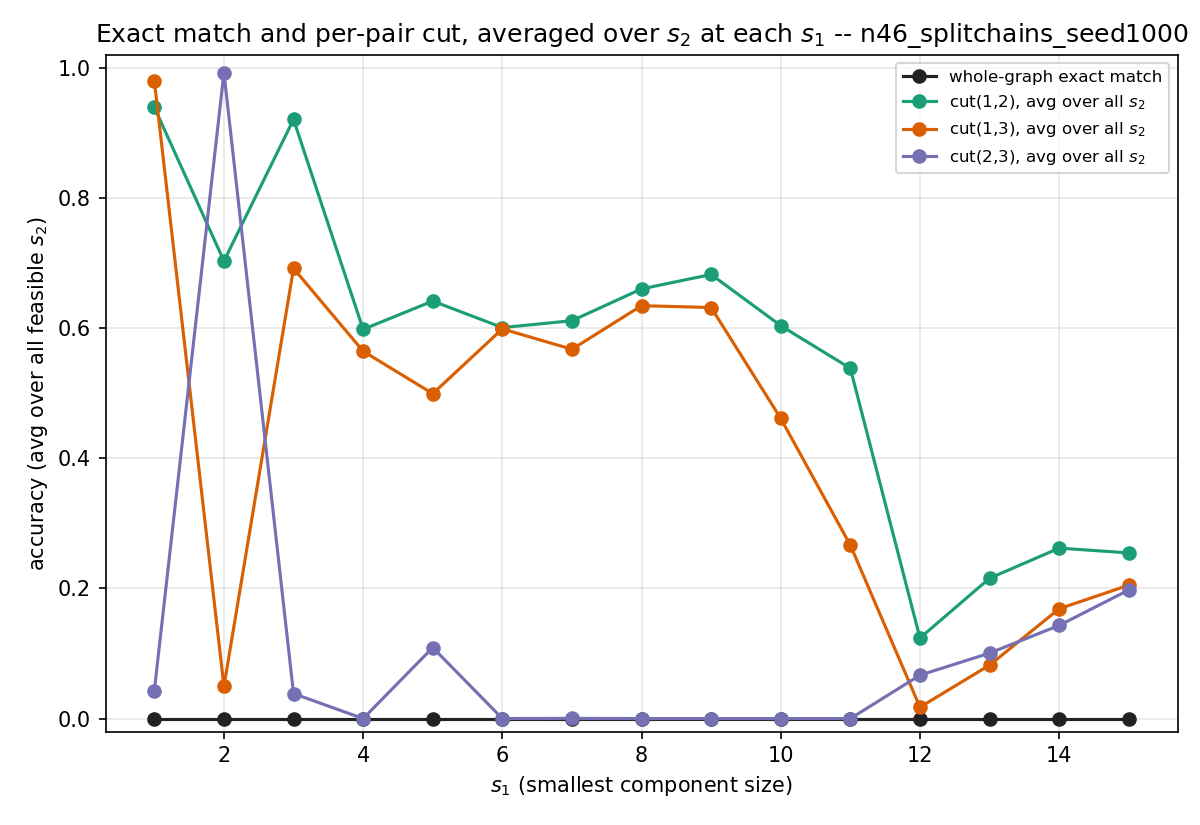
\includegraphics[width=0.75\textwidth]{figs/r9_threeway_exact_and_cut_by_s1_n46_splitchains_seed1000.png}
\caption{Exact match (always $0$) and each pairwise cut, averaged over every feasible $s_2$ at
each $s_1$. The cut(2,3) trace (purple) is near $1$ only at $s_1=1$, collapses immediately for
every $s_1\ge3$, and cut(1,3) (orange) is the one that is near $0$ instead at $s_1=2$ -- the
inversion of Headline 4.}
\end{figure}

\paragraph{Candidate cells for the next step (attention scores / layerwise cosine geometry) --
for the user to choose from.} A few natural candidates, spanning the qualitatively different
regimes above:
\begin{itemize}\setlength\itemsep{0.1em}
  \item $(s_1,s_2,s_3)=(1,22,23)$ -- the ``everything works except reach/cut noise'' case, the
        cleanest baseline with a trivial isolated node.
  \item $(s_1,s_2,s_3)=(4,15,27)$ or $(7,15,24)$ -- a typical ``2-out-of-3 cuts succeed, cut(2,3)
        fails'' cell, to see the mechanism behind Headline 3 directly.
  \item $(s_1,s_2,s_3)=(2,10,34)$ -- the $s_1=2$ anomaly (Headline 4), to see whether the
        inversion shows up as a visibly different attention/geometry pattern from the
        $s_1\ge3$ cells.
  \item $(s_1,s_2,s_3)=(15,15,16)$ -- the fully-balanced, everything-fails regime (Headline 5).
\end{itemize}

\subsection{Same test, on the 1chain+split\_chains checkpoint: cleaner, but the same core
story}

The identical $176$-cell sweep, unchanged, run against the OTHER $n{=}46$ seed-$1000$ checkpoint
that also never saw $3+$ components: the \S2 checkpoint trained on a $50/50$ mixture of a single
full chain ($k{=}1$) and random two-way splits ($k{=}2$). Whole-graph exact match is again
$0.000$ in all $176$ cells.

\begin{figure}[H]\centering
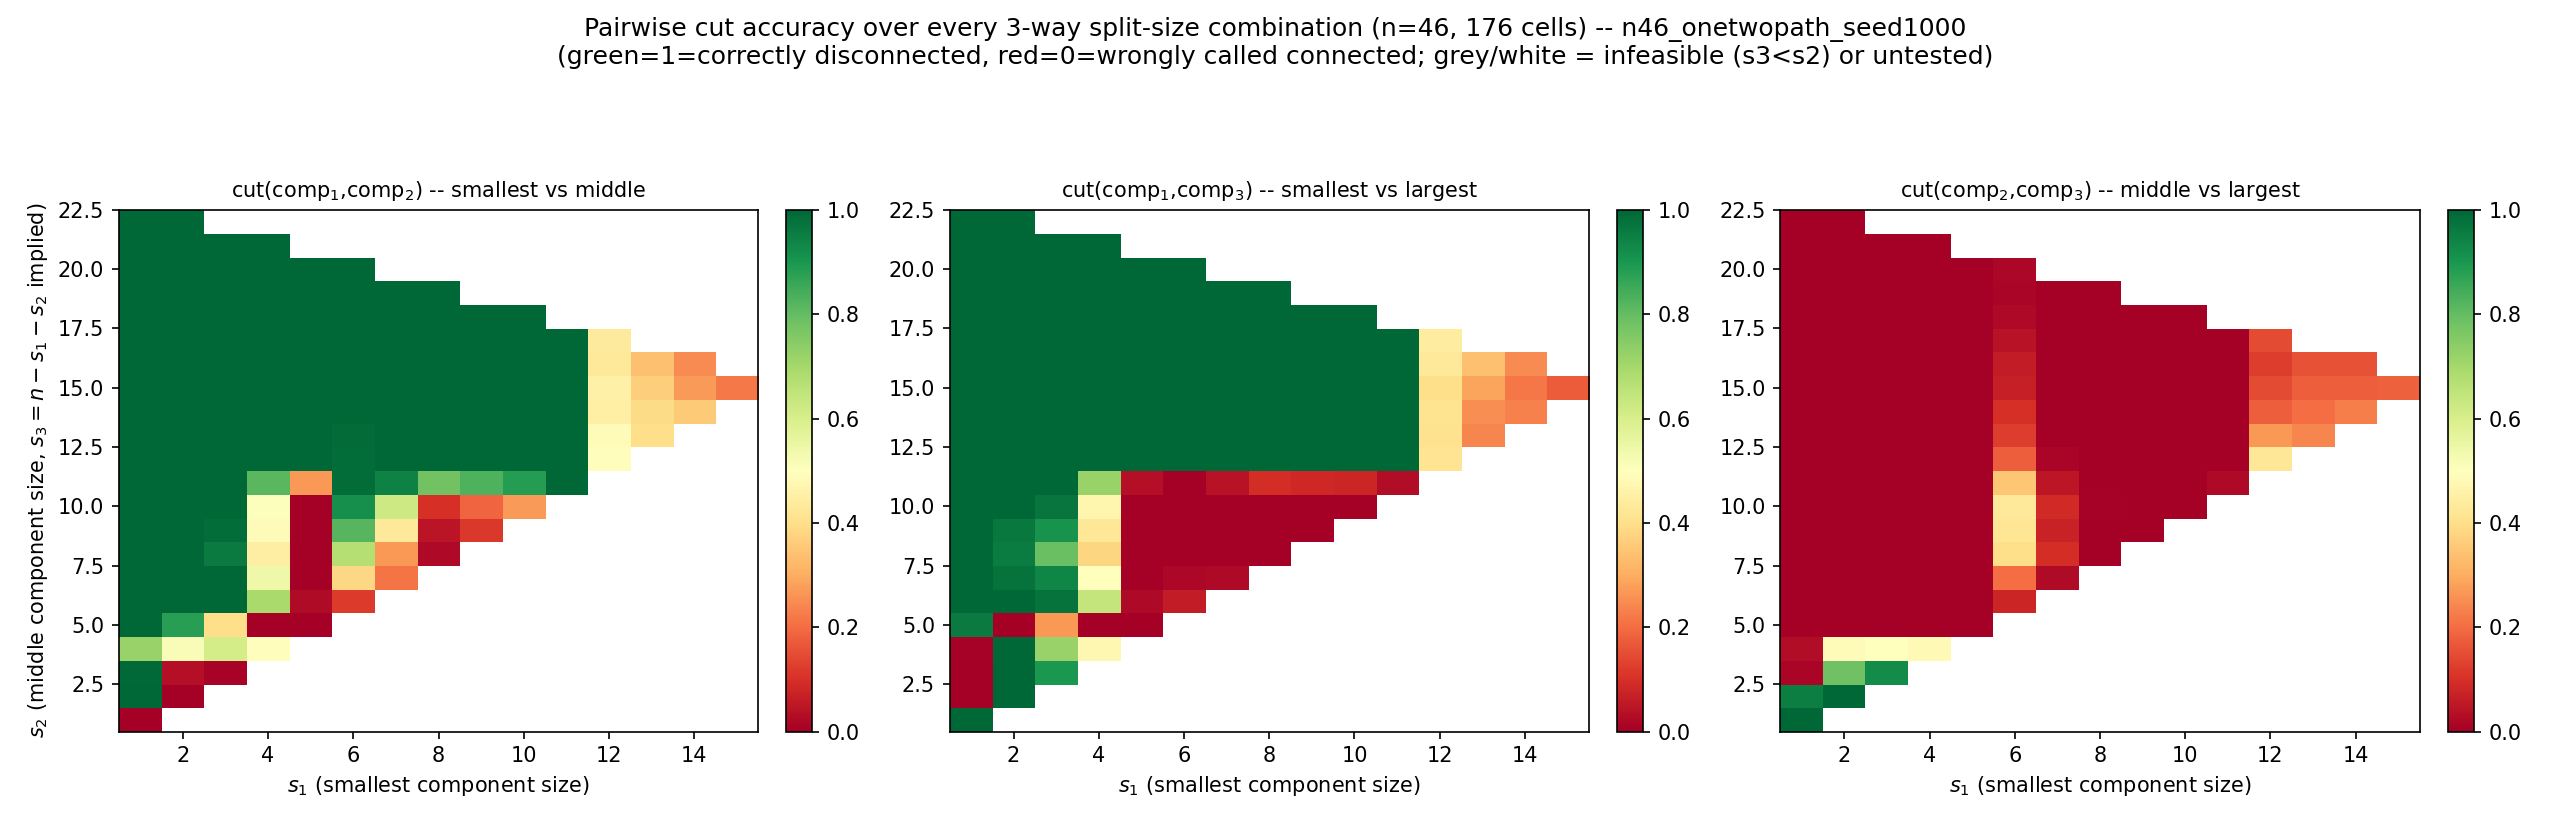
\includegraphics[width=0.98\textwidth]{figs/r9_threeway_cut_heatmaps_n46_onetwopath_seed1000.png}
\caption{Same three pairwise cut heatmaps as the split\_chains-only version above, on the
1chain+split\_chains checkpoint.}
\end{figure}

\paragraph{The core story is the same: cut(2,3) still fails almost everywhere.} The dominant
pattern is unchanged -- cut(comp$_2$,comp$_3$) (the two non-smallest components) is red (failed)
across almost the entire grid, exactly as for the split\_chains-only checkpoint.

\paragraph{But cut(1,2) and cut(1,3) are markedly more robust here.} For split\_chains-only,
cut(1,2)/cut(1,3) averaged (over $s_2$) only $0.5$--$0.7$ through most of $s_1=4$--$11$ and were
visibly noisy cell-to-cell. For 1chain+split\_chains, the SAME two cuts average $0.75$--$1.0$
across that entire range and stay high all the way out to $s_1=11$ (e.g.\ cut(1,2)$=0.999$ at
$s_1=11$, vs.\ only $0.538$ for split\_chains-only at the same $s_1$) -- a visibly cleaner,
wider green region in the heatmap above compared to Figure~15. Seeing single, un-split chains
during training (the $k=1$ case) appears to make the model noticeably better at telling a
non-trivial component apart from a small one, even though it still never saw 3 components.

\paragraph{The $s_1=2$ anomaly (Headline 4) does NOT replicate here.} For split\_chains-only,
$s_1=2$ inverted which pair fails (cut(1,3)$\approx0.05$, an outlier). For
1chain+split\_chains, $s_1=2$ is unremarkable: cut(1,3)$=0.947$, in line with its neighbours,
no inversion. This suggests the $s_1=2$ anomaly is a property of that specific checkpoint/seed,
not a general structural rule about single-edge components.

\begin{figure}[H]\centering
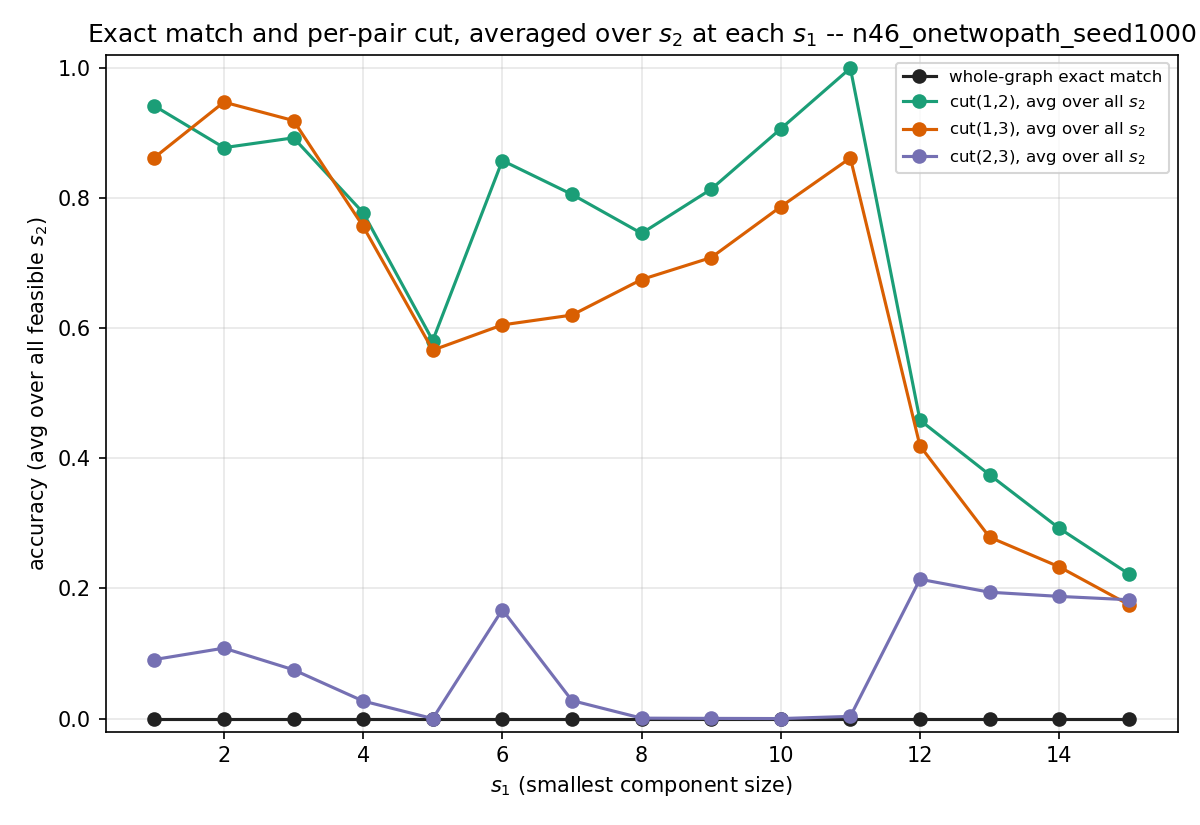
\includegraphics[width=0.75\textwidth]{figs/r9_threeway_exact_and_cut_by_s1_n46_onetwopath_seed1000.png}
\caption{Same by-$s_1$ summary as the split\_chains-only version above, on the
1chain+split\_chains checkpoint. Note cut(1,2)/cut(1,3)
(green/orange) sit visibly higher and smoother across $s_1=1$--$11$ than the split\_chains-only
version, and there is no dip at $s_1=2$.}
\end{figure}

\paragraph{Balanced-split degradation (Headline 5) still holds.} For $s_1\gtrsim12$ all three
cuts still collapse together here too (e.g.\ cut(1,2) drops from $0.999$ at $s_1=11$ to $0.459$
at $s_1=12$), just as for split\_chains-only.

\clearpage
\section*{Cross-experiment takeaways (one seed each --- read directionally, not definitively)}

\begin{enumerate}\setlength\itemsep{0.2em}
  \item \textbf{The endpoint-completion signal does not need the rich path\_union mixture.} Both
        narrower chain-based distributions (2-chains-only, 1+2-path) reproduce the identical
        break point ($a=12$) and the same qualitative reach-dip-then-recover shape as the full
        $1$--$4$-path mixture, with an equal-or-cleaner cut. If anything, the narrower
        distributions are \emph{more} robust on cut, not less --- the opposite of what one might
        expect if the phenomenon depended on having seen a wide variety of component counts.
  \item \textbf{Cycles, trained on properly, are NOT simply another counterexample to ``the
        diameter is the difficulty measure'' in the same way chains are.} They show a
        \emph{cleaner reach} (perfect at every split, no dip at all) but a \emph{much harsher cut
        failure} (exact, permanent $0$ rather than a soft floor) once the split is large enough.
        This is a genuinely different failure signature from every chain-based condition, not a
        milder or stronger version of the same one.
  \item \textbf{This speaks directly to the endpoints question.} Report~VIII's two-cycles test
        could not distinguish ``cycles are unlearnable'' from ``this model never saw a cycle at
        all.'' Training specifically and systematically on cycles removes that confound, and the
        cut \emph{still} fails totally past a threshold split -- so the earlier OOD collapse was
        not purely an unfamiliarity artefact. Whether this means path endpoints are strictly
        \emph{necessary} for the cut-sharpening mechanism, or whether cycles are simply harder in
        some other structural sense (every node locally identical, no distinguishing feature at
        the read-in step at all -- the candidate reading above), is not yet settled by a single
        seed and needs more seeds and probably more splits between $a=5$ and $a=12$ to pin down
        exactly where cut starts to go wrong.
\end{enumerate}

\section*{What is still missing before any of this becomes real Report IX content}
\begin{itemize}
  \item More seeds for all three conditions (this document is one seed each, by design --- see
        the warning box at the top).
  \item For the 2-cycles condition specifically: a denser split sweep between $a=5$ and $a=12$
        to locate the cut break point precisely (currently only $a=3,4,5,6,\ldots,11,12$ are
        covered, with a suspicious dip at $a=3$--$5$ worth a second look), and the candidate
        read-in-geometry explanation should be checked systematically (more splits, more seeds)
        before it is stated as anything more than a hypothesis.
  \item Only after that: fold the confirmed, multi-seed picture into the real Report~IX
        manuscript (Thread~A.2/A.5-adjacent for the chain-based results, Thread~B for the cycles
        result).
  \item For Thread~A.3 (the three-way split sweep): still purely behavioural on one seed --
        attention scores and layerwise cosine geometry are the deliberate next step, on
        whichever candidate cells above turn out to be of interest, before this becomes
        Report~IX content in its own right.
\end{itemize}

\end{document}
